%%
%% This is file `sample-acmsmall.tex',
%% generated with the docstrip utility.
%%
%% The original source files were:
%%
%% samples.dtx  (with options: `acmsmall')
%% 
%% IMPORTANT NOTICE:
%% 
%% For the copyright see the source file.
%% 
%% Any modified versions of this file must be renamed
%% with new filenames distinct from sample-acmsmall.tex.
%% 
%% For distribution of the original source see the terms
%% for copying and modification in the file samples.dtx.
%% 
%% This generated file may be distributed as long as the
%% original source files, as listed above, are part of the
%% same distribution. (The sources need not necessarily be
%% in the same archive or directory.)
%%
%% Commands for TeXCount
%TC:macro \cite [option:text,text]
%TC:macro \citep [option:text,text]
%TC:macro \citet [option:text,text]
%TC:envir table 0 1
%TC:envir table* 0 1
%TC:envir tabular [ignore] word
%TC:envir displaymath 0 word
%TC:envir math 0 word
%TC:envir comment 0 0
%%
%%
%% The first command in your LaTeX source must be the \documentclass command.
\documentclass[manuscript,screen,review,anonymous]{acmart}
\usepackage{emoji}

\usepackage{hyperref}
\usepackage{hyperxmp}
\usepackage[most]{tcolorbox}
\usepackage{lipsum}
\usepackage{xcolor}
\usepackage{multirow}
\usepackage{booktabs}
\usepackage{array}
\usepackage{rotating}
\usepackage{tabularx}
\usepackage{makecell}

\definecolor{linequote}{RGB}{224,215,188}
\definecolor{backquote}{RGB}{249,245,233}

\newtcolorbox{myquote}[1][]{%
    enhanced, breakable, 
    size=minimal,
    frame hidden, boxrule=0pt,
    sharp corners,
    colback=backquote,
    #1
}
% \documentclass[manuscript,review,anonymous]{acmart}
%% NOTE that a single column version is required for 
%% submission and peer review. This can be done by changing
%% the \doucmentclass[...]{acmart} in this template to 
%% \documentclass[manuscript,screen]{acmart}
%% 
%% To ensure 100% compatibility, please check the white list of
%% approved LaTeX packages to be used with the Master Article Template at
%% https://www.acm.org/publications/taps/whitelist-of-latex-packages 
%% before creating your document. The white list page provides 
%% information on how to submit additional LaTeX packages for 
%% review and adoption.
%% Fonts used in the template cannot be substituted; margin 
%% adjustments are not allowed.
%%
%% \BibTeX command to typeset BibTeX logo in the docs
\AtBeginDocument{%
  \providecommand\BibTeX{{%
    \normalfont B\kern-0.5em{\scshape i\kern-0.25em b}\kern-0.8em\TeX}}}

%% Rights management information.  This information is sent to you
%% when you complete the rights form.  These commands have SAMPLE
%% values in them; it is your responsibility as an author to replace
%% the commands and values with those provided to you when you
%% complete the rights form.
\setcopyright{acmcopyright}
\copyrightyear{2018}
\acmYear{2018}
\acmDOI{XXXXXXX.XXXXXXX}


%%
%% These commands are for a JOURNAL article.
\acmJournal{JACM}
\acmVolume{37}
\acmNumber{4}
\acmArticle{111}
\acmMonth{8}

%%
%% Submission ID.
%% Use this when submitting an article to a sponsored event. You'll
%% receive a unique submission ID from the organizers
%% of the event, and this ID should be used as the parameter to this command.
%%\acmSubmissionID{123-A56-BU3}

%%
%% For managing citations, it is recommended to use bibliography
%% files in BibTeX format.
%%
%% You can then either use BibTeX with the ACM-Reference-Format style,
%% or BibLaTeX with the acmnumeric or acmauthoryear sytles, that include
%% support for advanced citation of software artefact from the
%% biblatex-software package, also separately available on CTAN.
%%
%% Look at the sample-*-biblatex.tex files for templates showcasing
%% the biblatex styles.
%%

%%
%% The majority of ACM publications use numbered citations and
%% references.  The command \citestyle{authoryear} switches to the
%% "author year" style.
%%
%% If you are preparing content for an event
%% sponsored by ACM SIGGRAPH, you must use the "author year" style of
%% citations and references.
%% Uncommenting
%% the next command will enable that style.
%%\citestyle{acmauthoryear}

%%
%% end of the preamble, start of the body of the document source.
\begin{document}



%%
%% The "title" command has an optional parameter,
%% allowing the author to define a "short title" to be used in page headers.
\title{A Taxonomy of Gamified Prompt Elements for Enhancing Engagement with LLM Chatbots in Education}


% \author{Sai Siddartha Maram}
% \affiliation{%
%   \institution{University of California, Santa Cruz}
%   \streetaddress{}
%   \city{Santa Cruz}
%   \country{USA}}
% \email{samaram@ucsc.edu}


% \author{Magy Seif El-Nasr}
% \affiliation{%
%   \institution{University of California, Santa Cruz}
%   \streetaddress{}
%   \city{Santa Cruz}
%   \country{USA}}
% \email{mseifeln@ucsc.edu}


%%
%% By default, the full list of authors will be used in the page
%% headers. Often, this list is too long, and will overlap
%% other information printed in the page headers. This command allows
%% the author to define a more concise list
%% of authors' names for this purpose.
\renewcommand{\shortauthors}{Maram et al.}

%%
%% The abstract is a short summary of the work to be presented in the
%% article.
\begin{abstract}

Large Language Models (LLMs) are rapidly entering classrooms, offering personalized tutoring and feedback at scale. Yet, their interactions often remain transactional and uninspiring, limiting active engagement and deeper learning. Recent work suggests that framing LLMs as games can counter these limitations, but little is known about how to systematically design prompts that turn LLMs into effective game-based learning environments. This paper addresses that gap by introducing the notion of \textit{Gamified Prompts}—structured instructions that embed game elements such as narrative roles, progression systems, and challenge-response dynamics directly into LLM interactions. Through participatory design with educators, students, and researchers, we build a corpus of over 60 gamified prompts and, through thematic analysis, derive the first taxonomy of gamified prompt elements with 5 main dimensions. We evaluate this taxonomy in terms of coverage, usability, and the impact across various stakeholders. Our contributions provide a foundation for educators and designers to craft engaging, adaptive, and gameful learning experiences with LLMs.

\end{abstract}

%%
%% The code below is generated by the tool at http://dl.acm.org/ccs.cfm.
%% Please copy and paste the code instead of the example below.
%%
\begin{CCSXML}
<ccs2012>
   <concept>
       <concept_id>10003120.10003121.10003124</concept_id>
       <concept_desc>Human-centered computing~Interaction paradigms</concept_desc>
       <concept_significance>500</concept_significance>
       </concept>
 </ccs2012>
\end{CCSXML}

\ccsdesc[500]{Human-centered computing~Interaction paradigms}
%%
%% Keywords. The author(s) should pick words that accurately describe
%% the work being presented. Separate the keywords with commas.
\keywords{Game Mechanics, Serious Games, Religion, Input Modalities}

\received{20 February 2007}
\received[revised]{12 March 2009}
\received[accepted]{5 June 2009}

%%
%% This command processes the author and affiliation, and title
%% information and builds the first part of the formatted document.
\maketitle

\section{Introduction}
\label{introduction}
Large Language Models (LLMs) have become a transformative force in education, with chatbots from OpenAI, Google, and Anthropic increasingly integrated into classrooms—often free for students. LLM chatbots now assume diverse pedagogical roles including mentors, feedback providers, illustrators, peers, and digital teachers, offering real-time, personalized guidance \cite{mollick2023using}. This integration marks a critical shift, transforming technology from a static resource such as a digital textbook or learning management system into an active participant in the learning process \cite{shao2025strategies, maram2025listeninglanguagemodelsusing}. From an HCI perspective, their pedagogical value lies in creating interactive learning experiences, providing personalized scaffolding, self-paced learning environments, and fostering learner agency via immediate and non-judgmental feedback \cite{adiguzel2023revolutionizing,chen2023artificial,dwivedi2023opinion}.

However, this promise comes with significant limitations. LLM-based interactions are often described as transactional and repetitive, lacking the narrative richness or motivational framing required to sustain student engagement \cite{fenu2024exploring,gajos2022people,seo2021impact}. This transactional nature leads to LLMs providing accurate yet inert information, limiting deeper cognitive engagement and sustained learning \cite{achiam2023gpt}. Students may become passive recipients of AI-generated responses, reducing the active cognitive engagement necessary for deeper learning \cite{kooli2023chatbots}. Moreover, chatbots often produce generic, formulaic responses that fail to inspire creativity or critical thinking \cite{huang2022chatbots}, inadvertently promoting surface-level learning and reducing opportunities for students to develop unique perspectives or explore original ideas.

To address these concerns, researchers at the intersection of games and LLMs have proposed positioning LLMs as digital games, presenting educational concepts through digital game-based learning (DGBL) \cite{you2025enhancing,klopstock2025manchita,barmpari2025educational,wang2025effects}. By framing learning within interactive systems, games help students understand complex topics in meaningful contexts. Unlike traditional DGBL, which is often expensive, requires specific hardware, and relies on static, predetermined learning paths, LLMs enable ``adaptive contextual games" that are dynamic and responsive through. These LLM-powered games can analyze student performance in real-time to provide personalized feedback, customized hints, and tailored challenges that match individual learning styles and pace. Consider how an instructor might transform a simple climate change lesson into an engaging persuasion-based game as shown below:

\begin{quote}
    \textbf{Standard LLM Conversation}\\
    \textit{\textbf{Student}: How does afforestation help with climate change?}\\
   \textit{\textbf{LLM}: Afforestation helps combat climate change by capturing carbon dioxide (CO2) from the atmosphere through photosynthesis and storing it in tree biomass and soil. This process, known as carbon sequestration, reduces the concentration of greenhouse gases that contribute to global warming.}
\end{quote}

\begin{quote}
    \textbf{Gamified LLM Conversation }\\
   \textit{\textbf{LLM}: You are an environmental envoy meeting with the council of the town of Silverwood, a community historically dependent on industry. Your goal is to convince at least two of the three council members to support your afforestation initiative. You can speak to Mayor Thornton (pro-business), Farmer Ingrid (concerned about land use), or Elder Maeve (values tradition). Who will you approach first?}\\
   
   \textit{\textbf{Student}: I'll speak with Mayor Thornton.}\\
   \textit{\textbf{Mayor Thornton}: Welcome. I'll be blunt—my priority is jobs. This town was built on industry, and while I appreciate nature, I won't sacrifice our economic stability for a few trees. Explain to me how this 'afforestation initiative' benefits my constituents financially.}\\
   
   \textit{\textbf{Student}: Planting a new forest can create jobs in the short term for planting and maintenance, and in the long term, it can lead to sustainable timber industries and boost tourism. It's an investment in a new kind of economy for Silverwood.}\\
   
    \textit{\textbf{Mayor Thornton}: An interesting angle. You're talking about long-term economic diversification, not just an environmental project. I'm listening. However, Farmer Ingrid is worried you'll be taking over valuable agricultural land. How would you address her concerns?.}\\
\end{quote}

In this gamified scenario, the student transforms from passive information seeker to active ``environmental envoy" tasked with ``convincing" stakeholders. The abstract concept of ``afforestation" becomes a concrete quest embedded in the compelling game world of ``Silverwood," demanding strategic thinking and active participation.

However, this transformative potential introduces a critical challenge: the effectiveness of LLM-powered games depends on the quality of underlying instructions passed to the LLM \cite{atreja2025s,ma2025should,isaza2024prompt,cain2024prompting}—a skill known as prompt engineering. In the context of an educational game, this is far more complex than simply asking AI to ``make a quiz" or ``make a game." It requires designers to act as architects of learning experiences, carefully crafting detailed prompts that define the game's narrative, rules, goals, mechanics, and pedagogical strategy and also choosing where to give LLMs the creative liberty. We term such structured prompts which help creating gamified learning experiences via LLMs as ``Gamified Prompts".

While nascent research has proven LLMs' efficacy as games \cite{wang2025effects, shao2025strategies}, examined LLMs as educational NPCs \cite{barmpari2025educational,you2025enhancing}, and developed platforms integrating LLMs into game-based learning \cite{klopstock2025manchita,you2024gamifying}, our work addresses the foundational element: engineering prompts that enable LLMs to behave as gamified learning systems. Working with stakeholders in learning and education, we aim to introduce a taxonomy with dimensions that allow prompt designers, instructors, and game designers to integrate game elements into LLM-based learning experiences. We term this taxonomy as the ``Gamified Prompt Taxonomy". On that pretext, our core research question is: \textbf{What game design elements and strategies can be embedded into LLM prompts to enhance student engagement and learning outcomes in educational interactions?}

To address this, our paper makes the following scientific contributions:

\begin{enumerate}
    \item \textbf{A Corpus of Gamified Prompts:} We introduce a curated database of over XX gamified prompts co-designed with educators, students, and researchers. This is the first structured resource of its kind intended to support AI-enhanced classroom instruction through gamified interactions.

    \item \textbf{A Taxonomy of Gamified Prompt Elements:} Through thematic analysis of the corpus, we develop a design taxonomy that identifies key dimensions of gamified prompts such as narrative framing, feedback dynamics, challenge structure, and progression. This taxonomy provides educators and prompt designers with a conceptual framework for creating meaningful, engaging learning experiences with LLMs.

    \item \textbf{Evaluation of the Developed Taxonomy:} Apart from sharing the taxonomy, we also evaluate the taxonomy with regards to coverage, usability, and impact. 
    
\end{enumerate}

Through these contributions, we aim to provide a comprehensive framework for designing, understanding, and evaluating gamified interactions with LLM chatbots, fostering more engaging and effective learning environments.

\section{Previous Work LLMs for Education}

\subsection{LLMs for Education}
Large Language Models (LLMs), such as Claude, GPT-4o, and others, have demonstrated considerable potential in enhancing educational experiences. Trained on vast repositories of text data, these models possess extensive knowledge across a wide range of subjects, allowing them to answer questions, generate content, and support student learning in diverse educational contexts \cite{achiam2023gpt,uppalapati2024comparative}. As a result, educators and researchers have increasingly explored the integration of LLMs into classroom environments.

Language learning has been a prominent area where LLMs have shown considerable promise. Park et al. \cite{park2024align} and Koraishi et al. \cite{koraishi2023teaching} explored the use of LLM-powered chatbots to help students practice English language skills. These studies demonstrated how conversational agents effectively reinforce grammar, vocabulary, and conversational fluency by simulating real-world dialogue scenarios. Ye et al. \cite{ye2025position} emphasized that LLMs’ multilingual capabilities make them particularly effective tutors for Foreign Language Education (FLE). By adapting language complexity, providing translation assistance, and offering culturally relevant examples, LLMs create interactive learning environments that are tailored to individual learners. Furthermore, Zhang et al. \cite{zhang2024impact} explored how sustained chatbot interactions improved students' vocabulary acquisition and strengthened their command over linguistic structures. 


In addition to language learning, LLMs have shown remarkable potential in teaching computer programming and STEM subjects. Ma et al. \cite{ma2024teach} and Jin et al. \cite{jin2024teach} describe how LLMs assist students in debugging code by identifying errors, explaining code logic, and offering step-by-step guidance. Similarly, Tu et al. \cite{tu2023should} explored the integration of LLMs into data science instruction, where the models facilitated data analysis, generated synthetic datasets, and supported students in refining their code. Molina et al. \cite{molina2024leveraging} integrated LLM-based tutoring systems in computer science programming courses. Their study found that LLMs effectively supported learners by clarifying coding terminology, improving comprehension of complex programming concepts, and assisting in code debugging. By offering contextualized explanations and interactive coding guidance, LLMs have proven to be effective tools in enhancing computational thinking and problem-solving skills.


Beyond technical subjects, LLMs have been successfully employed to support creativity, critical thinking, and the humanities. Guo et al. \cite{guo2024prompting} demonstrated how LLMs helped students explore artistic concepts by generating visual descriptions, writing prompts, and creative ideas for design projects. Vastakas et al. \cite{vastakas2024cultural} and Trichopoulos et al. \cite{trichopoulos2023large} showed that LLMs effectively supported history education by generating timelines, simulating historical debates, and encouraging inquiry-based exploration. Chang et al. \cite{chang2025framework} demonstrated how LLMs can assist students in brainstorming project ideas, generating design concepts, and expanding creative possibilities. Similarly, Zha et al. \cite{zha2024designing} showed that LLMs effectively support project-based learning by co-creating ideas with students, offering design alternatives, and guiding students through iterative ideation processes. By engaging students in interactive dialogue, these tools encouraged reflection, deeper analysis, and creative problem-solving across diverse disciplines.

One of the most compelling strengths of LLM tutors is their ability to adapt to individual learners in real-time. Unlike static educational content, LLMs can assess a student's knowledge state, detect misunderstandings, and tailor responses accordingly \cite{meyer2024using}. For instance, if a student struggles with a particular mathematical step, an LLM tutor can break down the problem into simpler sub-tasks or provide targeted hints before gradually increasing the complexity as the student progresses. This dynamic personalization enables LLMs to support students in their optimal zone of proximal development \cite{pardos2024chatgpt}, ensuring content remains neither too difficult nor too simplistic.

The ability of LLMs to generate personalized feedback further enhances their value in educational settings. Studies such as those by Dai et al. \cite{dai2023can} and Jia et al. \cite{jia2022automated} demonstrate that LLM-generated feedback on essays, coding exercises, and short-answer questions closely mirrors the quality of feedback provided by human instructors. This immediate, specific feedback allows students to refine their work in real-time, fostering deeper learning. Similarly, Tanwar et al. \cite{tanwar2024opinebot} and Sessler et al. \cite{sessler2025towards} explored LLM-based systems that provide structured critique and targeted suggestions, improving students' ability to reflect, revise, and refine their ideas.




\subsection{Drawbacks of LLM-Based Education}

Despite their potential, LLM-based chatbots present several challenges in educational contexts. While these systems offer personalized feedback and scalable learning support, their effectiveness can be undermined by limitations in engagement, emotional connection, creativity, and pedagogical depth.

One major concern is the challenge of sustaining student engagement over time. Williams et al. \cite{williams2024ethical} and Fryer et al. \cite{fryer2020supporting} highlight that while LLM chatbots can initially capture students' interest due to their novelty and interactive nature, this enthusiasm often diminishes over time. Kooli et al. \cite{kooli2023chatbots} further argue that students may become passive recipients of AI-generated responses, diminishing the active cognitive engagement necessary for deeper learning. As interactions become predictable or transactional, students may disengage, reducing the chatbot’s educational value.

Kooli et al. \cite{kooli2023chatbots} also point out that LLM chatbots have limited capacity to foster genuine emotional and social connections in learning environments. Effective education often relies on empathy, encouragement, and trust — attributes that play a vital role in motivating students. While AI systems can simulate politeness or generate emotionally supportive responses, they lack true empathy and the nuanced understanding needed to form meaningful teacher-student relationships \cite{lin2024artificial}. Xiao et al. \cite{xiao2024review} reinforce this concern, noting that while chatbots can personalize content delivery and provide instant feedback, their emotional connection with students is inherently weaker than that of human educators. This absence of emotional rapport may reduce students' motivation, particularly for those who rely heavily on interpersonal support in learning environments.

Beyond emotional limitations, there are notable pedagogical concerns associated with LLM-based chatbots. Huang et al. \cite{huang2022chatbots} argue that chatbots often produce generic, formulaic responses that may fail to inspire creativity or critical thinking in learners. While chatbots excel at generating structured explanations or feedback, the uniformity of these responses can inadvertently promote surface-level learning. For instance, if students consistently receive similar AI-generated essay feedback, this homogeneity may reduce opportunities for students to develop unique writing styles or explore original ideas. Cenry et al. \cite{vcerny2023educational} observed that students often described conversations with chatbots as transactional and repetitive, resulting in reduced immersion and engagement. Similarly, Hellas et al. \cite{hellas2024experiences} and Lauricella et al. \cite{lauricella2023ludic} found that students reported chatbot interactions as monotonous and uninspiring, with AI responses often feeling mechanical and lacking the depth required for reflective learning.



\subsection{Prompt Engineering for Education}

The preceding sections illustrate how LLMs can support both students and instructors by offering personalized guidance, feedback, and interactive learning opportunities. However, to effectively leverage these capabilities, instructors must carefully design prompts that guide the behavior of popular LLMs such as GPT-4, Claude, and other models. The process of constructing such prompts raises the question: how can instructors streamline the behavior of these LLMs to align with their educational objectives?

The answer lies in Prompt engineering i.e the process of crafting effective prompts. Prompt engineering has emerged as a crucial skill for educators and learners interacting with AI systems \cite{spasic2023using, cain2024prompting}. Instructors increasingly rely on prompt engineering to dictate how LLMs respond, what content they focus on, and how they engage with students \cite{hedderich2024piece, wu2022ai, allen2023use}. A prompt may range from a simple instruction, such as “Explain Newton’s laws in simple terms,” to more complex multi-part directives that outline step-by-step guidelines for the chatbot’s behavior \cite{pando2024prompting}. The structure, wording, and detail within these prompts significantly impact the quality and relevance of the AI’s responses \cite{walter2024embracing, mollick2024instructors}. Consequently, mastering prompt engineering has become a key skill for educators seeking to integrate LLMs effectively into their teaching strategies.

Due to the critical role of prompt design, there is growing interest in exploring strategies for crafting effective prompts and training educators in these techniques \cite{park2024generative, eager2023prompting, wang2023unleashing}. One emerging strategy is prompt chaining, which involves breaking complex tasks into a series of smaller, sequential prompts. Each subtask’s output feeds into the next prompt, effectively creating a multi-turn pipeline to handle complex objectives. Sun et al. \cite{sun2024prompt} highlight how prompt chaining enables LLMs to handle sophisticated tasks, such as analyzing a student's essay and then generating customized quiz questions based on that analysis. This technique reduces cognitive overload for the LLM, making it easier for educators to achieve their intended outcomes. Cain et al. \cite{cain2024prompting} emphasize the value of iterative prompt engineering, arguing that prompts refined through repeated testing and revision tend to produce more reliable and contextually appropriate responses. Iteration allows educators to refine their prompts by adjusting language, tone, or instructions to ensure improved engagement and better alignment with their learning objectives.

Given that effective prompt engineering can be time-consuming and challenging, researchers have increasingly developed resources to support instructors in this process. Lan et al. \cite{lan2024teachers} highlight that the responsibility for crafting prompts often falls on instructors, many of whom lack formal training in AI-driven educational tools. To address this, researchers have proposed structured frameworks that guide prompt creation. Lo et al. \cite{lo2023art} introduce a four-step framework designed to help educators create effective prompts. This framework emphasizes that prompts should (a) be precise, (b) provide clear context, (c) specify desired output formats, and (d) control the length and complexity of language. Such structured approaches empower educators to design prompts that yield coherent, informative, and contextually appropriate responses.

Similarly, Velasquez et al. \cite{velasquez2023prompt} present the Goal-Prompt-Evaluation-Iteration (GPEI) model. This framework follows four stages: (a) establishing the learning goal, (b) designing the prompt, (c) evaluating AI-generated responses, and (d) iterating on the prompt based on evaluation results. By following this structured process, instructors can refine their prompts to improve response accuracy, pedagogical alignment, and student engagement.

To further support educators, several online repositories and educational platforms now provide curated databases of effective prompts. Resources such as Learning Prompting\footnote{\url{https://learnprompting.org}}, ChatGPT Educational Resources\footnote{\url{https://openai.com/index/teaching-with-ai/}}, and specialized MOOCs on prompt engineering for educators\footnote{\url{https://www.coursera.org/specializations/prompt-engineering-for-educators}} offer practical guidance and sample prompts that instructors can adapt for their classrooms. Additionally, some LLM-powered tools, such as the Prompt Professor\footnote{\url{https://chatgpt.com/g/g-qfoOICq1l-prompt-professor}}, are designed to help educators construct effective prompts by suggesting improvements and refining prompt wording.

Beyond these tools and frameworks, researchers have also established databases and taxonomies of prompt templates to help instructors address common instructional challenges. MacNeil et al. \cite{macneil2023prompt} argue that using predefined prompt templates can alleviate design, language, and time-related barriers that instructors often face when developing prompts from scratch. Zamfirescu et al. \cite{zamfirescu2023johnny} further highlight that prompt templates provide a structured starting point for instructors, especially when navigating unfamiliar pedagogical contexts. By offering adaptable templates, these resources empower instructors to efficiently construct effective prompts while addressing common challenges such as vague instructions, overly complex language, or ambiguous output expectations.

Mollick et al. \cite{mollick2023assigning, mollick2023using} propose a comprehensive taxonomy of AI use cases in educational settings, including AI-tutors, AI-coaches, AI-mentors, AI-teammates, AI-tools, AI-simulators, and AI-students. Their taxonomy is supplemented by a curated prompt library that educators can use as a foundation for creating AI-driven learning experiences\footnote{\url{https://www.moreusefulthings.com/instructor-prompts}}. While this library does not critically analyze the design components of prompts, it serves as a valuable starting point for instructors seeking to experiment with prompt-driven educational strategies.

In addition to broad educational contexts, domain-specific frameworks are emerging to support instructors in specialized fields. Olla et al. \cite{olla2024ask} introduce a taxonomy of healthcare-related prompts designed to support medical educators in crafting context-specific LLM interactions. Similarly, institutions such as Harvard\footnote{\url{https://www.huit.harvard.edu/news/ai-prompts}} and UC Davis\footnote{\url{https://guides.library.ucdavis.edu/genai/prompt}} have developed educational resources that provide prompt templates tailored to specific academic disciplines.




\subsection{LLMs for Game Based Learning}

A promising approach to mitigating these engagement, emotional, and pedagogical challenges is integrating playful and gamified elements into chatbot interactions. Historically, games for learning utilizing conversational agents faced limitations from fixed responses and restricted natural language capabilities \cite{gobl2021conversational,fadhil2017adaptive,othlinghaus2017supporting,jeuring2015communicate}. However, recent advancements in AI and LLMs offer significant potential for developing dynamic, narrative-driven, and playful educational chatbots \cite{bonetti2024using}. Huber \citep{huber2024leveraging} that game-based learning via LLMs not only harness the creative affordances of LLMs but are best positioned not as authoritative tutors but as gamemasters that co-construct rules, scenarios, and reflective debriefs, thereby shifting the pedagogical emphasis from static delivery to procedural co-creation.

This positioning is evident in role-playing simulations, where Stampfl \textit{et al.} demonstrate how students can engage in civic or professional dialogues with ChatGPT as a simulation partner \citep{stampfl2024role,stampfl2024revolutionising}. Their work highlights not only the increased immersion such systems afford but also the way the LLM’s improvisational capacity encourages deeper negotiation of meaning. Tódová \textit{et al.} \cite{todova2025quest} show how LLM-driven NPCs can sustain open-ended dialogue that maintain immersion and challenges students to think from multiple perspectives. Unlike traditional scripted NPCs, these characters embody misconceptions, ethical stances, or stakeholder perspectives that are central to inquiry-based learning, thereby expanding the epistemic role of NPCs from mere quest-givers to dialogic interlocutors.

In counselor education, Maurya \citep{maurya2024qualitative} show how ChatGPT can play the role of a client, allowing trainees to practice counseling strategies in low-stakes but realistic conversations. Breen \citep{breen2025large} experiments with historical simulations push this further, where LLMs generate branching character briefs that enable more nuanced explorations of past dilemmas . Kindenberg \textit{et al.} \cite{kindenberg2025role} building on role-playing note that LLMs reconfigure the design space for historical games by making adaptive scenario generation feasible within curricular constraints.

Beyond the use of LLMs as NPCs, Chen et al. \cite{chen2025characterizing} introduced an LLM platform that supports student learning through interactive storytelling. In addition to generating narratives, this chatbot provides visual content to enhance the storytelling experience. LLMs, with their extensive knowledge bases, have also simplified the creation of quiz games \cite{sreekanth2023quiz}. These quiz-games facilitate interactive narratives, allowing students to advance through levels or respond to progressively challenging questions while actively engaging with the chatbot \cite{sweetser2024large}.

Steenstra et al. \cite{steenstra2024engaging} presented a system that teaches adolescents about health education through an interactive narrative, where both the storyline and visual elements are generated by LLMs. Students are asked to select the right answer for questions generated by the LLM. Likewise, Caraco et al. \cite{caraco2025scaffolding} developed a chatbot-style game in which the LLM assigns programming and IT design tasks to help students enhance their system architecture skills. These studies collectively demonstrate promising results, illustrating how LLM-based chatbot games can support student learning via simulating real world scenarios. Zhang \textit{et al.} \cite{zhang2024simulating} take the logic of simulation further in their work on SimClass, a system where LLM-powered agents assume the roles of teachers and students to mirror classroom dynamics. Their studies show that multi-agent simulations help learners rehearse discourse strategies and anticipate peer responses, effectively creating a game of classroom participation. 

The literature clearly establishes LLMs as engines for playable pedagogy that enable role-play, NPC immersion, classroom simulations, and quest-based assignments to expand game-based learning possibilities. Early evidence demonstrates gains in engagement and higher-order thinking, which naturally leads instructors, researchers, and educational game designers to ask: "How do I build a gamified LLM?" or "How do I prompt an LLM to behave like a game?" All LLM-based chatbot games share a common feature—they use prompts to guide chatbot behavior. However, existing research lacks structured, detailed exploration into how specific game mechanics can optimally embed within LLM prompts. While educational applications of LLMs widely employ traditional tutoring, mentoring, and Socratic methods, a significant gap remains in understanding precisely how instructors can leverage game elements and mechanics to impact learner motivation, critical thinking, and other benefits that previous authors have identified.

Our research addresses this critical gap by systematically exploring game mechanics suitable for integration into LLM prompts and providing educators and instructional designers with structured tools for creating gamified chatbot interactions. We acknowledge the benefits of gamified LLMs for learning that previous authors have demonstrated and extend existing work by proposing a comprehensive gamified prompt taxonomy that categorizes effective design elements. This taxonomy enables instructors to develop targeted, playful, and pedagogically sound chatbot interactions while we examine both creator and learner perspectives. Our investigation explores how prompt designers perceive the usability of our taxonomy while simultaneously measuring how learners respond in terms of motivation, critical thinking, and situational interest compared to traditional and Socratic chatbot methods. Through this integrated approach, we offer both theoretical insights and practical tools for educators seeking to harness the potential of playful, LLM-driven learning interactions while addressing current limitations in the field.




\begin{figure}
    \centering
    \includegraphics[width=\linewidth]{images/Group 96.png}
    \caption{Participant involvement across taxonomy development and evaluation phases. Activities span generative co-design, prompt collection, taxonomy construction, and evaluative studies measuring coverage, usability, and learning impact.}
    \label{fig:participant_involvement}
\end{figure}




\begin{figure}[!ht]
    \centering
    \includegraphics[width=\linewidth]{images/Group 232 (1).png}
    \caption{(a) The architecture and API calls that support StudyHelper. (b) StudyHelper Playground: A platform to create prompts and test prompts. (c) StudyHelper Taxonomy Mode: A platform to explore the gamified prompt taxonomy, create prompts and test prompts. (d) An illustration of how prompt creators can use the Gamified Prompt taxonomy while creating gamified prompts.}
    \label{fig:StudyHelper}
\end{figure}


\section{Methodology}

As mentioned in Section \ref{introduction}, the aims of the paper, are (a) Develop a corpus of gamified prompts, (b) Develop a taxonomy from the corpus of gamified prompts and (c) Evaluate the taxonomy with regards to converage, usability and impact. For developing the corpus and evaluating the usability we used a tool called StudyHelper. Our methodology took multiple steps to meet the above objectives as illustrated in Figure \ref{fig:participant_involvement}. 


\subsection{Understanding StudyHelper:}
Before detailing each step outlined above, we provide a comprehensive overview of StudyHelper to establish context for readers. StudyHelper comprises two complementary platforms: StudyHelper Playground (Figure \ref{fig:StudyHelper} (b)) and StudyHelper Taxonomy Mode (Figure \ref{fig:StudyHelper} (c)). Both modes support designers in iteratively refining chatbot prompts, in this case on gamified educational interactions, while facilitating seamless collaboration between prompt creators and students.

\subsubsection{Prompt Creation in StudyHelper PlayGround:} As shown in Figure \ref{fig:StudyHelper} (a), StudyHelper leverages OpenAI's GPT-4o model as its core language processing engine, but distinguishes itself from conventional ChatGPT interactions through its systematic use of explicitly user-defined prompts to guide dialogues and also initiating the conversation. For instance, consider Figure \ref{fig:methodsIllustrations} (right), here we notice how StudyHelper automatically introduces initiates the conversation through an introductory message based on the underlying prompt. This architectural design ensures that all interactions remain precisely aligned with specific educational objectives and pedagogical goals. As illustrated in Figure \ref{fig:StudyHelper} (b) there exists a panel wheres users can enter their prompt instructions and click ``Create Custom GPT" to interact with their created prompt. All iterations are automatically stored in a secure backend database, enabling creators to revisit, modify, iterate and build upon their previous work over time. 

\subsubsection{Prompt Creation in StudyHelper Taxonomy Mode}: The StudyHelper Taxonomy Mode extends StudyHelper Playground enabling prompt creatprs to explore the proposed gamified prompt taxonomy. Prompt creators, educators, and researchers can access this comprehensive taxonomy by selecting ``View Taxonomy" (Figure \ref{fig:StudyHelper} (c)), which provides detailed access to various taxonomical dimensions, theoretical descriptions, and practical examples of constituent elements (Figure \ref{fig:StudyHelper} (d)). This taxonomy serves as both a reference guide and an inspiration source for prompt creators, helping them systematically incorporate evidence-based gamification principles into their educational chatbot designs.

\subsubsection{Student Interaction:} From the student perspective, learners can access StudyHelper and interact with a curated library of prompts created by instructors and prompt designers. Importantly, all student interactions with these prompts are systematically logged and stored in the backend system for future analysis. 

\subsubsection{Current Limitations of StudyHelper:} The implementation of StudyHelper used as part of the current study has certain limitations. First, the maximum allowed prompt length is 7000 words. This was deliberately chosen to optimize performance. Next, prompt creators did not have the ability to choose what model they wanted and were only allowed to use GPT-4o from OpenAI for this study. 


For readers seeking a deeper understanding of StudyHelper's architecture, user interface, and pedagogical applications, we strongly recommend reviewing the supplementary video material and exploring the interactive platform at [URL REDACTED for Review].

\begin{figure}
    \centering
    \includegraphics[width=\linewidth]{images/Group 239 (2).png}
    \caption{(left) Poster used to advertise Hackathon to use StudyHelper to create bots. (middle) Participants interacting and comparing various bots. (right) Instruction Slides given to participants to participate in class assignments}
    \label{fig:methodsIllustrations}
\end{figure}


\subsection{Contribution 1: Constructing a Corpus of Gamified Prompts:}

In the generative step of our research, we utilized StudyHelper Playground. 
Using the Playground, we organized three participatory activities to develop a corpus of prompts. These stakeholders for these activities were chosen to include a diverse group of creators with varying skill-sets such as Human Centered Design, Game Design and pedagogy. The generative process consisted of (a) Co-Design session with instructors, (b) Hackathon among HCI and Game Design Students, (c) Workshops among Game Design Students. 


\subsubsection{Co-design with Instructors:} Through co-design sessions with three instructors, we developed four gamified prompts that the instructors considered highly suitable for their classrooms. All the three instructors were familiar with game based learning, have had previous research experience, teaching experiences and publication experiences with regards to game based learning and self-reported to use AI regularly. The sessions were organized over Zoom, where instructors were given a demo of StudyHelper, and requested to create gamified prompts, instructors were free to iterate and test these prompts as part of the co-design sessions. In the co-design sessions, we included engineers to support any technical or AI related queries, researchers from learning sciences to engage in discussions regards to pedagogy and researchers associated with game mechanics to support discussions with regards to game mechanics. The prompts generated as a result of this co-design processes, revolved around topics such climate change, statistics, tech ethics, and research design.

\subsubsection{Gamified hackathon among HCI and Game Designers:}
While the instructor led prompts are critical for understanding pedagocial integration with LLM based gameplay, we recognize students are critical stakeholders for the success of gamified prompts for learning. To gather their perspectives and approach towards gamified prompts, we organized the Gamified hackathon, a competitive event hosted within the HCI and Game Design department of <A LARGE PUBLIC UNIVERSITY>. 

We aimed to gather leverage the expertise of senior graduate students in game design and HCI who have taken extensive coursework with regards to AI and Design, AI and Games. The skill set of this group of participants allowed us to capture perspectives both from a Human Centered Design perspective, and Game Design perspective. The hackathon encouraged participants to creatively develop and design educational bots of their choice, by embedding engaging game mechanics and design practices. Participants actively used the Playground in StudyHelper to prototype, test, and refine their prompts. From this hackathon we generated 16 gamified prompts across a wide variety of topics like literature, finance, ethics, journalism, physics and many more. To ensure appropriate motivation, and high quality prompts the gamified hackathon had a prize money of \$50,\$30,\$20 for the first, second and third prizes.

\subsubsection{Gamified Prompt Creation Assignments:}
To gain further prompts, and students perspective, we embedded a gamified prompt creation assignment into two Game Design courses at <A LARGE PUBLIC UNIVERSITY>. The students were senior game design students, with all participants claiming to have developed at least 2 digital games as part of their coursework. The first class, consisted of 45 students and the class had a focus on AI, Games and UX of AI. The second class consisted of 6 students, and the class had a specific focus on developing games for change using AI. The assignments, after the discussion with the respective instructors were embedded into their classroom program to allow students to practically apply game design principles, AI design principles which were part of their cousework, in developing educational chatbot games. By directly involving students, game designers, and designers in the generative process, we ensured the resulting prompts accurately reflected the elements that participants themselves found engaging and motivating. From this exercise, we collected 40 prompts. 


Overall, from the co-design activity, gamified hackathon and university assignments, we received a total of 60 gamified prompts. The different activities to build our corpus ensured we got a diverse range of participants, prompts across a broad range of topics, game design elements and pedagogical approaches. 




\subsection{Contribution 2: Building the Taxonomy:}
\label{taxonomyBuilding}


The taxonomy aims to help instructors and prompt creators by: (a) providing designers with game elements game mechanics to embed in their prompts, (b) offering examples on how the identified game elements and mechanics can be embedded into their prompts.


\begin{figure}
    \centering
    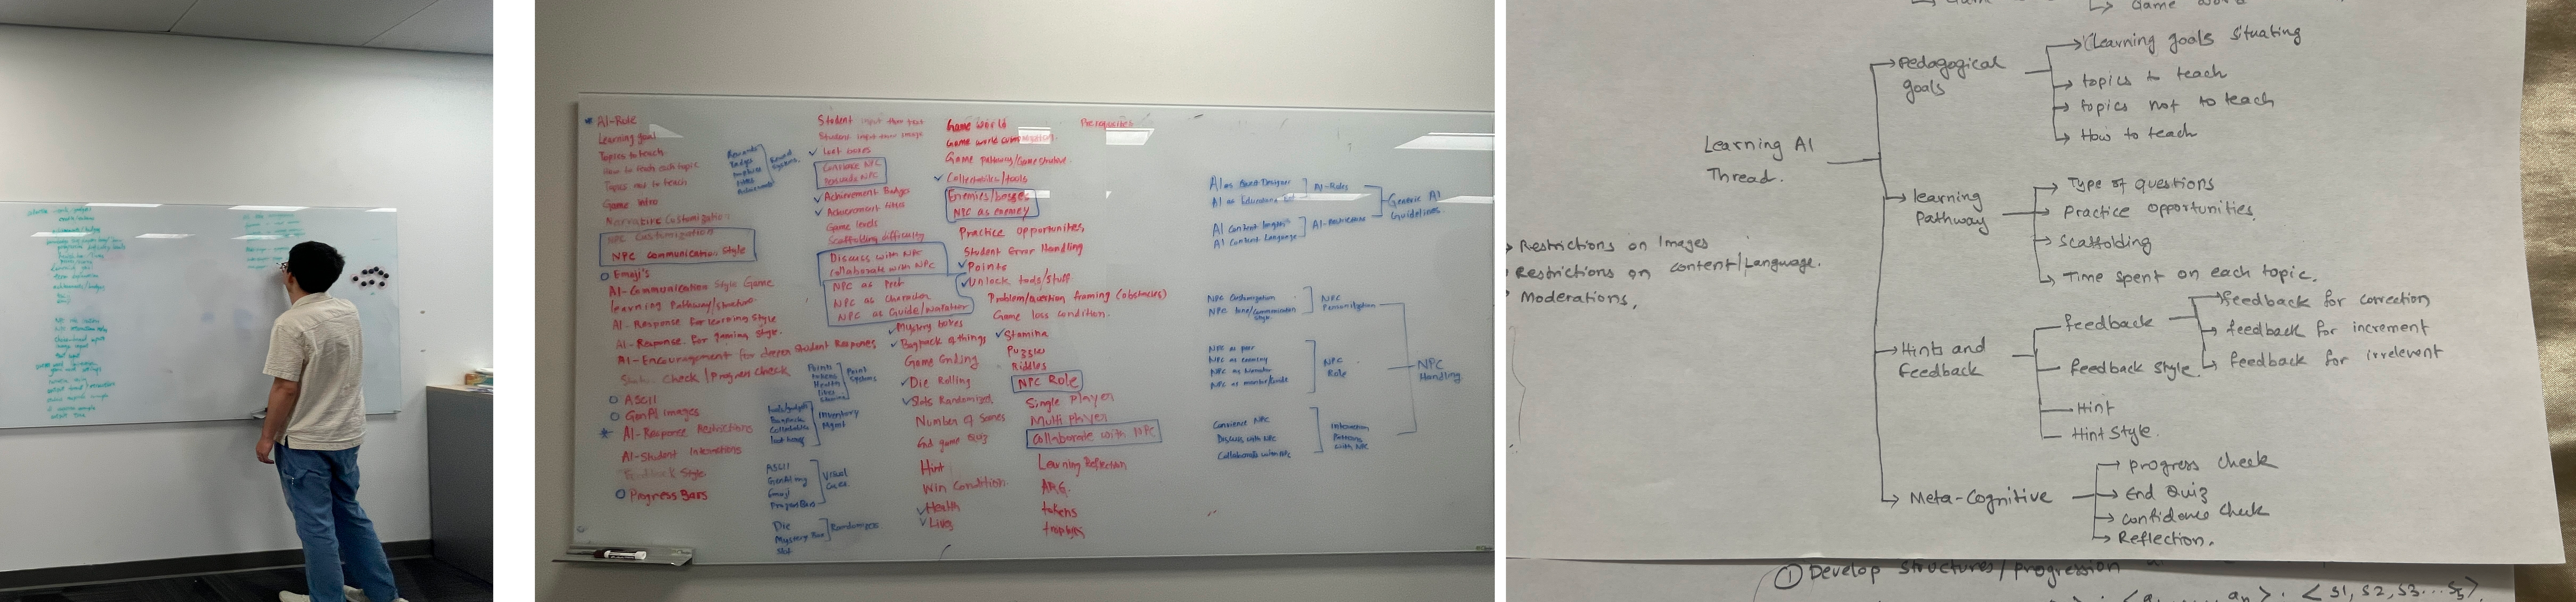
\includegraphics[width=\linewidth]{images/Group 199.png}
    \caption{Researchers developing the dimensions of the taxonomy through an iterative process}
    \label{fig:codebook-gen}
\end{figure}

The analysis began with two researchers applying a grounded theory approach \cite{maram2022astraverse,charmaz2006constructing} to uncover key dimensions within the corpus of gamified prompts. One researcher first segmented the prompts into fine-grained units, guided by thematic shifts and ensured that each unit captured a coherent idea or design element for subsequent analysis. The researchers then engaged in multiple collaborative sessions as illustrated in Figure \ref{fig:codebook-gen}. In this session the researchers, reviewed the dataset, interacted directly with the prompts, and iteratively refined the segmentation. They used constant comparison and memoing to discuss emerging themes and gradually constructed a codebook encompassing open, axial, and selective codes. In the early stages, the codebook contained a broad set of open codes, which the researchers collapsed and reorganized through axial coding to highlight relationships among design choices, pedagogical strategies, and game mechanics. Selective coding then identified higher-level categories that reflected overarching dimensions in the dataset.

To establish reliability, both researchers independently coded 30\% of the dataset using the shared codebook. They calculated inter-rater reliability (IRR) with Cohen’s Kappa and iterated on code definitions until they reached an IRR of 0.78, a threshold widely considered acceptable \cite{landis1977measurement,maram2024ah}. After achieving this level of agreement, the lead author independently coded the remainder of the dataset.

\subsection{Contribution 3: Evaluating the Taxonomy:}
\label{taxEval}

To rigorously assess our gamified prompt taxonomy, we draw on established principles from taxonomy evaluation literature, particularly within information systems \citep{Nickerson2013method,Kaplan2022introducing,Pinto2024automatic} and HCI \citep{Tabassi2023aiuse,jeoung2025promptprism,maram2022astraverse,maram2023visual}. We operationalize this assessment through three core constructs: \textbf{Coverage}, \textbf{Usability}, and \textbf{Impact}. These constructs are widely recognized as essential for evaluating knowledge organization systems. They ensure the taxonomy is comprehensive in scope and accurately represents the domain (Coverage) \citep{Pinto2024automatic, Mokkink2018cosmin, Nickerson2013method}, is practical, learnable, and efficient for its intended users (Usability) \citep{Pinto2024automatic, Tabassi2023aiuse, TaxonomyStrategiesUsability, Das2017human}, and is demonstrably beneficial in improving the quality of outcomes derived from its use (Impact) \citep{Bowman1999interaction}. Our approach aligns with methodologies that emphasize empirical testing and user-centered evaluation to validate the overall quality and utility of a taxonomy \citep{maram2023visual, Das2017human, Kaplan2022introducing}.


\begin{figure}
    \centering
    \includegraphics[width=\linewidth]{images/Group 229 (1).png}
    \caption{The Gamified Prompt Taxonomy illustrated with examples, and all the levels of codes.}
    \label{fig:GLPTax}
\end{figure}


\begin{itemize}
\item \textbf{Coverage: } We evaluated coverage to determine whether our taxonomy provides a comprehensive, accurate, and relevant representation of the diverse range of gamified elements and strategies that designers can embed within prompts \citep{Pinto2024automatic, Nickerson2013method, Kaplan2022introducing}. Specifically, we sought to verify that any gamified prompt, regardless of its complexity or specific gamified nature, can be appropriately situated and classified within the taxonomy's structure. To assess this coverage, we conducted a Game Design-AI workshop where we invited game designers to construct gamified prompts without prior exposure to our taxonomy. Since we intend the taxonomy as a design support tool rather than a fixed curricular framework, testing it with participants skilled in design thinking and creativity provides meaningful insights into its coverage and robustness \cite{sanders2008co,deterding2011game}.
All participants had either completed or were actively enrolled in game design and advanced game design courses. Each participant reported building a portfolio of at least three games previously. This background equipped them with the ability to creatively generate prompts, identify mechanics, and test the taxonomy's adaptability across diverse scenarios. However, in future iterations, we also plan to conduct detailed workshops with faculty and instructors. The workshop generated a total of 21 distinct prompts. Using the taxonomy we developed in the generative step, researchers mapped elements from the taxonomy to corresponding elements in all 21 prompts.

\item \textbf{Usability (Ease of Creation and Guidance)}:A major objective for the taxonomy's construction was to ensure it serves as an efficient and helpful tool for users—specifically faculty, instructors, and designers—in the process of creating gamified prompts \citep{jeoung2025promptprism, TaxonomyStrategiesUsability}. To evaluate this, we invited 34 stakeholders. The stakeholders consisted of 5 active instructors, 7 Teaching Assistants (who were also researchers), and 22 junior game designers who self-reported to have built atleast 2 functional games in the past, and have experience with AI and Games. This study employed a within-subjects design, where each participant created gamified prompts under two randomized conditions: once without the taxonomy and once with its aid. Participants first independently developed a gamified LLM prompt using the StudyHelper's playground (See Figure \ref{fig:StudyHelper} (b)) and then completed a second task utilizing the proposed taxonomy through the StudyHelper’s ``Taxonomy Mode," which was designed to help users systematically explore and apply gamified elements (See Figure \ref{fig:StudyHelper} (c) and (d)) \citep{TaxonomyStrategiesUsability, jeoung2025promptprism}. All participants recruited for these sessions self-identified as being familiar with LLMs and prompt engineering.

Following these tasks, stakeholders completed the NASA-TLX (Task Load Index) \citep{hart1988development} and TAM (Technology Acceptance Model) \citep{davis1989technology} surveys. These instruments were specifically chosen to provide a comprehensive picture of usability. The NASA-TLX allowed us to measure the perceived workload of the creative task itself, assessing dimensions like mental demand, effort, and frustration. This was crucial for quantifying whether the taxonomy made the process less cognitively demanding. In parallel, the TAM survey evaluated the users' perception of the taxonomy as a tool, focusing on its Perceived Usefulness (Does it help me create better prompts?) and Perceived Ease of Use (Is the taxonomy itself easy to apply?). Together, these measures allowed us to assess both the efficiency of the task (via NASA-TLX) and the potential for long-term adoption of the taxonomy (via TAM).

\item \textbf{Impact (Improved Prompt Quality)}:  To measure the impact of our proposed taxonomy, we evaluated it from the perspectives of two key stakeholders: prompt creators and end-users. From the prompt creators, we gathered qualitative insights following the usability test (see above paragraph) where participants answered open-ended questions about their experience. This approach allowed us to understand the taxonomy's role in their prompt creation process and to identify which aspects they found most, or least, impactful in supporting the design of instructional prompts.

From the students perspective, we hypothesized that an effective taxonomy should enable instructors to design prompts that students find more engaging and immersive. To test this, we conducted an experiment with 10 players who interacted with prompts on two topics: climate change and basic math. For each topic, participants were presented with three distinct prompts representing varying levels of design sophistication. The first was a control prompt, a standard instructional prompt created without any taxonomy guidance. The second was a gamified prompt developed without our taxonomy, while the third was a gamified prompt created by instructors who utilized our taxonomy. Throught the paper, we refer these three prompts as Level 0 (L0), Level 1 (L1), and Level 2 Prompts (L2). Participants first ranked the prompts based on the overall quality of their interaction. Furthermore, to obtain quantitative measures of the underlying psychological experience, participants completed specific subscales from three validated instruments. To assess immersion and engagement we used the designated immersion and engagement questions from the Player Experience of Need Satisfaction (PENS) \cite{ryan2006motivational}. We measured enjoyment, a core component of intrinsic motivation, using the Interest/Enjoyment subscale of the Intrinsic Motivation Inventory (IMI) \cite{ryan1983relation}. Finally, to gauge cognitive absorption and focus, we used the Attention Quality subscale from the Situational Interest Survey \cite{linnenbrink2010measuring}. The selection of these specific subscales allowed us to precisely target and measure key indicators of a highly engaging and immersive user experience.  
\end{itemize}








\section{Results}
In this section, we discuss evidences to our contributions based on the above methodology. We first present the gamified prompt taxonomy i.e. the different topics of prompts, we present the taxonomy itself, where we share all the identified game design elements and its implementations via prompts, the distribution of dimension elements across prompts. Finally, we present the evaluation of the taxonomy on metrics such as coverage, usability and impact.

\begin{figure}
    \centering
    \includegraphics[width=\linewidth]{images/Group 241.png}
    \caption{(left) Number of Gamified prompts made across various learning topics. (right) Density of taxonomy elements distributed across the corpus of gamified prompts.}
    \label{fig:distributions}
\end{figure}






\subsection{Contribution 1: The Gamified Prompt Corpus}
Through our various prompt generation activities we obtained a total of 60 prompts. As illustrated in Figure \ref{fig:distributions}, these prompts were distributed across topics such as Programming, STEM (math, physics, chemistry, statistics, probability), Life skills (cooking, healthcare, farming, banking), Research and Ethics(research methods, ethical research), Climate and Environment (climate change, ocean cleanup), Humanities (literature, history, art), and other various topics. 

For the larger community benefit, we publicly share all the gamified corpus prompts online at [URL REDACTED FOR REVIEW], and the can also be found in the webpage attached in the supplementary files. As illustrated in Figure \ref{fig:corpusPromptExample}, for each gamified prompt in the corpus, we tag it with all the game design elements found in the prompt, further users who wish to interact with the taxonomy, can also interact with the taxonomy by clicking the ``Interact" option. 

\begin{figure}
    \centering
    \includegraphics[width=\linewidth]{images/Group 243 (1).png}
    \caption{A prompt from the gamified prompt corpus with appropriate codes highlighted. As illustrated the corpus website [URL Redacted for review], will allow users to search, query prompts based on tags, and will allow users to interact with the prompts.}
    \label{fig:corpusPromptExample}
\end{figure}


The average length of the prompt was 394 words, with 43 prompts being under 500 words, 10 prompts between 500-750 words, 2 prompts between 751-1000 words and finally, 5 prompts between 1001-1500 words. To identify dimensions with the gamified prompt corpus, we split each prompt into granular units to faciliate in the taxonomy development. To guide the division of prompts into granular units, the rationale we took is to answer the question was the answer to ``This part of the prompt asks the LLM to ....". Everytime we identified a unit in the prompt that instructed LLMs to behave in a certain way we marked it as a unit of analysis. In Figure \ref{fig:corpusPromptExample}, we presented highlighted sections of individual units which were used for subsequent analysis. Overall, we identified 960 units to analyze across 60 prompts. As illustrated in Figure \ref{fig:distributions} we notice a majority of prompts had 10-19 analyzable units. In the following steps, we discuss the outputs of analyzing these units i.e. the taxonomy itself. 


\begin{figure}
    \centering
    \includegraphics[width=\linewidth]{images/Group 245 (1).png}
    \caption{(a) An ARG styled game, where participants are requested to upload labels of food products to discuss and analyze with the LLM, (b) A prompt suggesting the LLM to generate images when there is a shift in the game world, (c) Points and Visualization of the Point System through ASCII character.}
    \label{fig:argPromptExample}
\end{figure}





\begin{figure}
    \centering
    \includegraphics[width=\linewidth]{images/Group 244 (2).png}
    \caption{(a) A multiplayer game collecting user name (names changed for anonymity) and role, (b) Titles and Achievements to motivate players, (c) The use of randomization in the form of die rolls within the gameplay.}
    \label{fig:multiPlayerPromptExample}
\end{figure}




\subsection{Contribution 2: Core Taxonomy Structure }
%- What and How can gamified elements be integerated into prompts?
Using the above units, we developed the taxonomy through a grounded theory approach as detailed in the Section \ref{taxonomyBuilding}. As illustrated in Figure \ref{fig:GLPTax}, the taxonomy encompasses five selective codes: \textbf{Game Mechanics}, \textbf{AI Control}, \textbf{The Teacher}, \textbf{Game Director}, and \textbf{NPCs}. Each selective code contains multiple axial codes that further decompose into specific open codes, creating a hierarchical structure. In this section, we discuss each selective code, and underlying axial and open codes. 

\subsubsection{The Game Director}

The \textbf{Game Director} selective code encompasses the structural elements that define how gamified learning experiences unfold over time. The \textbf{Game Type} axial code reveals diverse approaches to player interaction, ranging from regular single-player games, to more complex multiplayer and ARG framings. While within the corpus, while most gamified bots are regular single player games, we noticed a few, we noticed some games encouraged more then one player interacting with the chatbot at once. In this situation the AI serves as the moderator, dictating whose turns and tasks for each player. In a gamified bot aiming to teach Ethical Journalism, the designer incorporates an element of mulitplayer by including the following in the prompt - \textit{``First ask all the names of the players and assign them roles. Assign roles to each player like the Boss, Journalist, Social Media Influencers. For each turn, give [....]"}, an interaction for for this prompt is illustrated in Figure \ref{fig:multiPlayerPromptExample} (a). Given the ability to comprehend images, we noticed few gamified prompts encouraging users to submit images to progress in the game. For instance, a programming based game stated - \textit{``Have users submit, hand written code and provide feedback after analyzing the hand written code".} On a similar tangent as illustrated in Figure \ref{fig:argPromptExample} (a), a gamified bot aiming to teach sugars and ingredients mentioned - \textit{``In this challenge, give specific tasks, prompting students to upload food label images [....]".} The ability to comprehend images and providing learning tasks which requires users to interact with the real world, blurs boundaries between the AI game space and real world, resulting in ARGs i.e. Alternate Reality Games. 

The \textbf{Game Conditions} selective code is responsible for establishing clear win and loss states that provide closure and introduction to the game. A bot teaching Statistics, defines success in their prompt - \textit{``mastery demonstrations of statistical concepts needed for exam preparation by the player finish all the interactions with the NPC.''} while a chatbot teaching probability through a haunted house narrative, creates explicit failure conditions where \textit{``losing all three lives ends the exploration experience.''}. The establishment of winning and loosing states is crucial to inform the players of their gaming goals, and to determine when to stop the game. 

The \textbf{Game Pathway} axial code structures the temporal flow of learning experiences through carefully designed introductions, level progressions, and culminating activities. A bot teaching climate change exemplifies pathway design with its elaborate introduction - \textit{``You have been chosen to join the Guardians of Earth, a secret league dedicated to protecting our planet''} followed by progressive challenges that increase in complexity. Essentially the Game pathway, provides structure in terms of how to start the game, how to progress the game and finally, how to end the interaction in the game. 

The \textbf{Game World} elements create immersive contexts that situate learning within compelling fictional environments. For instance, a bot aiming to teach probability and finance, situates user in Las Vegas as a Casino host - \textit{``You are to act as a Casino host for a roulette game in the MGM at Las Vegas, taking in all the possibilities for a single 0 roulette game [...]"}. Similarly, another prompt aiming to teach players about Python programming illustrates this by placing the player in space - \textit{``The theme of this lesson is `Stranded In Space' where the user is trapped inside of a spaceship. They will need to get the spaceship into working shape and navigate it back to Earth."} Similarly, as illustrated in Figure \ref{fig:corpusPromptExample}, the user is allowed to choose their own world, and the LLM crafts the NPCs and narratives according to the selected game world. 

\subsubsection{Game Mechanics}
The \textbf{Gameplay Mechanics} selective code represents the most recognizable aspects of gamification, encompassing the reward systems, mechanics, and visual elements that transform educational interactions into game-like experiences. The \textbf{Reward/Points System} axial code emerges as a central motivational structure, manifesting through achievements, badges, trophies, titles, and point systems that provide immediate feedback and recognition for learning progress. \textbf{Achievements} function as milestone markers that recognize specific learning accomplishments. For instance, in a prompt titled `Stats Quest \emoji{movie-camera}' the designer incorporates a tiered achievement system, where player is awarded titles by adding the following lines - \textit{``if the student identifies the hypothesis correctly, award them the `Hypothesis Hero' recognition, and for proper statistical testing, give them `Analysis Expert'.''}. 

Apart form the use of titles we noticed the use of \textbf{Trophies, Badges and Medals} to provide immediate feedback, and gratification for students. For instance, in a gamified prompt aiming to teach climate change, we saw the designer prompt - \textit{``Provide the Gaurdian, a Bronze Medal \emoji{3rd-place-medal} for basic environmental awareness, Silver Medals \emoji{2nd-place-medal} for implementing conservation strategies, and Gold medals \emoji{1st-place-medal} for designing comprehensive sustainability solutions."} This tiered medal systems, titles creates clear progression pathways while recognizing different levels of mastery within the same conceptual domain. 


\textbf{Points systems} take advantage of the memory function of chatbots. Previous scores/points are stored in memory of the chatbot, and when a player takes an action in chat, corresponding manipulation is done to the points. For instance, in a gamified bot aiming to teach literature, the designer incorporates a weighted point system by including the following line in the prompt - \textit{``have a weighted point system, where players are awarded more points for deeper analysis of the character, rather then surface level observations"}. Essentially providing an opportunity for students to engage more thoughtfully with literary texts. Similarly, as illustrated in Figure \ref{fig:multiPlayerPromptExample} (b), as users finish various tasks they are awarded with points which also result in them receiving specific badges. 

An other engaging way to create immersion and engagement was the use of Survival systems. The \textbf{Survival System} introduces risk and consequence elements through \textbf{health}, \textbf{lives}, and \textbf{stamina} mechanics that add urgency and strategic thinking to educational interactions. A gamified prompt aiming to teach Probability situated in a haunted house, demonstrates this approach by stating in their prompt \textit{``The player gets 3 lives, and they can progress through rooms as long as they can"}. Similarly, a gamified prompt named ``Math Dungeon" employs health points, where they include the following in their prompt - \textit{navigate the dungeon, where each problem answered wrong reduces health points, the adventurer can recover health points when they meet Dr.Pythogres}.


\textbf{Inventory Management} systems create persistent engagement through collectible items, tools, and resources that students accumulate and utilize throughout their learning journey. This again takes into account the memory functionality of chatbots, where the memory stores items and tools the players have been given or gathered as part of their progression. In a gamfied bot aiming to teaching sugars and food ingredients, the designer incorporates tools that the users can use, by including the following line - \textit{``Allow the players to pull any of the detective tool to find hidden sugars in the image"}. Further, in a climate change game the designer mentions - \textit{``Form the climate armory, allow users to choose the \emoji{water-pistol} Plasma Shooter, \emoji{sponge} Pollution Sponge, to tackle the climate catastrophe"}. Similarly, as illustrated in Figure \ref{fig:multiPlayerPromptExample} (c), the user is provided options to add an item into their inventory or not deciding their fate in the next level. These inventory systems transform abstract learning progress into tangible, manipulable assets that students can strategically deploy.


The last approach towards leveraging LLMs as part of gameplay, was the use of randomization as a mechanics. For instance, in a game that users move across a board to encounter various puzzles at different steps, the designer mentions \textit{``Use a custom die roll to decide how many steps the player can move forward."} Building on randomization mechancis, we saw designers also introduce loot Boxes, slot machines and mystery boxes to add an element of surprise and have the gameplay adjust based on the items recieved in the boxes. For instance, in a game teaching finances provided opportunities for players to gamble money in slot machines and illustrate how it could be a bad practice - \textit{``players are allowed to spend money on a slot machines, allow them insert their money in multiples of 10".} Simillarly, in Figure \ref{fig:multiPlayerPromptExample} (c), we notice how the player is provided with a die role whose outcomes determines the fate of the player as they navigate a dungeon.

\subsubsection{The Teacher}

The \textbf{Teacher} selective code contains the educational elements that make these prompts effective learning tools. This is where game mechanics meet actual teaching and learning goals.

The axial code \textbf{Pedagogical Goals} define what students should learn and how they should learn it. The pedagogical goal part of the prompt is what instructs prompts the LLM on \textbf{Topics to teach}, \textbf{Topics not to teach} and information on \textbf{How to teach the topic}. In the corpus, there exists a prompt, which aims to teach Math foundations, the prompt contains - \textit{``Your goal it to teach students foundations of Mathematics."}. Next, a bot teaching Climate change explicitly mentions to focus on certain topics while avoiding other topics - \textit{``Make sure the discussion revolves around scientific facts on causes of climate change and not political debates about climate change".} This ensures, the LLM is situated to teach only topics the instructors want the students to learn. Similarly, as illustrated in Figure \ref{fig:corpusPromptExample}, the instructor apart from mentioning what topics to teach (t-tests, ANOVA) also advises the LLM to stay away from topics such as two-way ANOVA and Chi-square. By instructing the LLM on what topics to teach and not to teach, the designer ensures the experience of learning is aligned to the goals of the class or instructor. 

The \textbf{Learning Pathways} axial code captures how the prompt designers aims to sequence learning material within the game. For instance, a chatbot aiming to teach players permutations and combinations through Blackjack stated - \textit{``First explain the different cards in a playing deck, and the number of cards, [...], explain the definitions of permutations and combinations, use the cards to show the examples. Encourage players to explain their thinking.} Here we notice, the step-by-step approach to provide granular information instead of feeling overwhelmed by difficult concepts too early. In another bot, aiming to teach programming for children the prompt mentions - \textit{I want at least 3 interactions for each level. Before the interaction takes place, have the NPC provide some information on the topic of the level so the student can be given information about the topic before being presented a challenge. Please do not print out the entire level into one response. If the player gets stuck allow the student to ask the NPC for the level to help them out. Do not directly tell the student how to clear the encounter until they have asked for help at least 3 times.} The prompt clearly lays out the structure in terms of how they want the students to interact with the bot and how the LLM should present its learning goals. Such structured approach is also evident in Figure \ref{fig:multiPlayerPromptExample} (b), where the bot first introduces the concept of variables, and then moves onto arithmetic operations. 

\textbf{Hints and Feedback} systems help students when they are stuck in a particular task, or provide corrective measures when students get answers to questions wrong. For instance, in a prompt aiming to teach students research methods, the prompt guides students to think about the correct approach instead of having the prompt directly provide answers to questions they answer wrong - \textit{``When students give a response, ask them to explain their reasoning before going to the next question, however if they get an answer wrong, instead of giving the answer, provide hints that help them think critically and reach the answer."}

The \textbf{Metacognitive} elements in the prompt help students think about their own learning. In the corpus, a bot aiming to teach research methods regularly checks-in with students about how confident they feel about different research concepts, and also if they are ready to move on to the next segment in the game - \textit{``After reach section, ask students how confident they feel in the section, ask them to rate their confidence between 1-5. If they share a low confidence score, gather information with that the student is not confident about and provide more examples on the topic."} This is also evident in Figure \ref{fig:corpusPromptExample}, where users are requested to rate their confidence before moving on to the next confidence. Other approaches, which designers have used to provide reflection on their learning includes asking players to summarize their experience and reflect on their experience. For instance, in a bot aiming to teach Aztec history, the participants are asked to share a summary of their gameplay at the end of the session - \textit{``After the last level, ask players to reflect on the various NPCs and summarize their conversations and strategies used to expand their empire". }


\subsubsection{AI Control}

The \textbf{AI Control} selective code addresses the technical and procedural aspects of AI behavior that ensure consistent, appropriate, and effective interactions. The \textbf{Output Control} axial code are instances in the prompt, that guide the output of the AI responses. For instance, across iterations, we noticed participants found the AI responses to be long and verbose, to counter this, designers often included - \textit{``Keep your response between 200 to 400 characters"}. To illustrate this difference, consider Figure \ref{fig:multiPlayerPromptExample} (a) and (b), The first prompt requests the LLM to keep the response limited to 150-300 characters, resulting in shorted LLM responses, while the second prompt does not mention any such restriction, resulting in the LLM providing longer responses. Further, we noticed to ensure educational appropriateness and while maintaining game narrative authenticity designers placed Language restrictions, and output moderation ensuring images generated, and text generated is educational and does not digress from the main topic.

The \textbf{Input Control} axial revels approaches to how player interact with AI systems. While we already discussed the ability of gamified chatbots to interpret images, and how they can be used by players to submit images, photographs and even hand written texts. Apart from images and regular text based input, other input mechanics included  \textbf{Choice-based input systems} where students are provided with a set of options which they are free to choose from. For example, in a gamified chatbot aiming to teach about sustainable fishing practices, the designer mentions - \textit{``Let users choose among the following options for their fishing camp \emoji{keycap-1} Lake Fork, \emoji{keycap-2}, [....]"}. This is also evident in Figure \ref{fig:argPromptExample} (b), where users are provided an option to choose which aspect of the game world they want to explore.

Apart from text, LLMs have taken strides in generating image. Given this advantage to make the game experience more playful, designers took advantage by incorporating \textbf{Visual elements} in AI responses. Visual elements provide immediate aesthetic feedback through multiple modalities that transform text-based interactions into rich sensory experiences. In a prompt titled the Physics Dungeon, the user uses \textit{ASCII} as a form of art to create mazes - \textit{``Create 10×10 matrix visual representations using ASCII characters to show the dungeon layout, player position, and discovered pathways.''}. An illustration of this is also evident in Figure \ref{fig:argPromptExample} (c), where the task of the user is to climb a tower and the tower is demonstrated using ASCII. Similarly, we notice in Figure \ref{fig:argPromptExample} (b) how various scenes as described in the prompt are illustrated to the users to situate the users within the game world.

\textbf{Emojis} serve dual functions as both aesthetic enhancement and information encoding systems. A prompt titled Climate Quest employs emojis - \textit{``\emoji{earth-africa} Climate Quest,'' ``Welcome, Explorer! \emoji{earth-americas}\emoji{sparkles}''}  as consistent symbolic representations of different environmental concepts. Emojis's apart form helping frame the game world, also help in providing clarity on other design elements. For instance, survival mechanics such as hearts, powers and collectible were also represented by emojis, a gamified bot teaching, physics clearly instructed -  \textit{``Always place the Health Bar (10 hearts) at the start of the message and the Progress Bar at the end... Health: \emoji{heart}\emoji{heart}\emoji{heart}\emoji{heart}\emoji{heart}\emoji{heart}\emoji{heart}\emoji{heart}\emoji{heart}.''} Similarly, the \textit{Statistics Quest} explicitly encouraged visual tracking of player progress: \textit{``Highlight progress of players using emojis and a progress bar like Progress: [\emoji{rocket}\#\#\#\#\#] 10\%.''} To highlight the difference, consider Figure \ref{fig:multiPlayerPromptExample} (c) where the prompt creator does not include emojis, resulting in conversations without the emoji's while other prompts within Figure \ref{fig:multiPlayerPromptExample}, Figure \ref{fig:argPromptExample} and Figure \ref{fig:corpusPromptExample} the explicit mention of Emoji's results in emoji's within LLM's responses.



% For starters, We notice how designers define various \textbf{AI Roles}, these are different from NPCs created as part of the game. AI Roles defined how the LLM presents itself within the gamified environment beyond an NPC. For instance, the AI can take the role of an AI educator, AI quest designer or an AI practice bot. In a bot teaching programming, the designer incorporates the following - \textit{``You are a friendly and fun fantasy adventure narrating bot to help kids learn about the basics of coding. Your goal is to create a fun and engaging chat adventure that will serve as an introduction to simple coding concepts to kids."} Here the role of the bot is a AI fantasy narrating bot, with a specific tone as established by the prompt creator. 
% during their environmental missions. In another bot teaching ethical dilemmas the designer incorporates - \textit{``You are a gamified chatbot that generates interactive narratives centered around ethical dilemmas"}, explicitly mentioning the LLM to be a gamified chatbot. 


\subsubsection{Non-Playable Characters}

The \textbf{NPC Establishing} selective code addresses the creation and management of non-player characters that populate gamified learning environments. This code also encompasses the customization options and communication styles that make artificial characters feel authentic and engaging. A climate quest gamified bot mentions - \textit{``diverse Guardian characters with distinct personalities who communicate using different expertise areas."} Further, we noticed, prompt designers giving players create their own NPCs through tone and role, a gamified bot aiming to allow users practice for interviews mentions - \textit{``ask users what they want the interviewer to interview them on, allow them to choose the difficulty and tone of the interviewer, allowing them to practice and simulate all scenarios.} Similarly, A literature teaching bot, positions certain NPCs as \textit{``literary characters from the studied works who engage students in dialogue about themes and symbolism,''} creating peer-like interactions with fictional entities. A statistics teaching bot employs NPCs - \textit{``friendly mentors who provide encouragement and hints when students struggle with statistical concepts."}

\textbf{Interaction Patterns with NPCs} structure the types of engagements students have with artificial characters, including conflict resolution, persuasion scenarios, collaborative problem-solving, and discussion facilitation. A prompt aiming to teach students reserach methods creates collaborative NPCs where \textit{``students must convince artificial stakeholders about their research design choices"}, requiring persuasive communication skills alongside methodological knowledge.












\subsection{Contribution 2.1: Structural Dependencies, and Relations Between Taxonomy Dimensions}

\begin{figure}
    \centering
    \includegraphics[width=\linewidth]{images/Screenshot 2025-08-26 at 13.07.24.png}
    \caption{Co-Ocurrance Matrix of all the 19 axial codes. Each cell indicates the number of prompts a particular axial code has appeared.}
    \label{fig:coocurance-matrix}
\end{figure}


In the above sub-sections, we discuss individual dimensions in the taxonomy, and the impact of the taxonomy for creation. In this section, we discuss the how various dimensions across the taxonomy are related and what we can learn from them. First, we develop a co-occurance matrix as illustrated in Figure \ref{coocurance-matrix}. This matrix indicates the number of prompts that contain a particular axial code. 

\subsubsection{The Game Pathway Connector Hub:} As shown in Figure \ref{fig:coocurance-matrix} Game Pathway dominates the network as the central organizing principle, appearing in 53 of 60 prompts (88.3\%) and maintaining the strongest co-occurrence relationships across the taxonomy: Game World (38 prompts, 63.3\%), Output Control (34 prompts, 56.7\%), Pedagogical Goals (33 prompts, 55.0\%), AI Roles (33 prompts, 55.0\%), and NPC Role (31 prompts, 51.7\%). To best understand this hub-like connectivity, we can look at a gamified prompt that aims to teach Shaksphere Literature in the corpus.
In this gamified prompt the Game Pathway (``players journey through three difficulty levels: Beginning, Intermediate, and End-Game") co-occurs with Game World (``players feel like they are living inside the book"), Pedagogical Goals (``teach literature through immersive gameplay"), NPC Role (``fictional characters who guide, challenge, or interact"), and Output Control (``generate a narrative response describing the player's journey"), demonstrating how progression mechanics serve as the structural backbone connecting all design elements. 

The co-occurrence patterns also revel design dependencies that beyond simple frequency analysis. For instance, the Inventory Management axial code demonstrates near-complete dependence on Game Pathway infrastructure, co-occurring in 18 of its 19 appearances (94.7\% conditional probability). For instance, in a gamified prompt in the corpus, students are tasked with ``making various potions, using herbs collected across levels". This illustrates how the inventory can not function without the underlying progression structure. Similarly, NPC Role shows 96.9\% dependence on Game Pathway, visible in a chemistry gamified prompt, where the prompt mentions ``at least one NPC character should help the player at each quest". These asymmetric relationships—where specialized elements require Game Pathway but Game Pathway functions independently—suggest a generative hierarchy rather than a flat taxonomy. 

Byoned the game pathway, Figure \ref{fig:coocurance-matrix} also exposes natural element clusters: pedagogical elements show strong mutual co-occurrence. For instance, in a game teaching climate change, the prompt contains, Learning Pathway (``Explain real-world environmental impacts at various habitats"), Pedagogical Goals (``Teach players about climate change"), and Hints And Feedback (``Provide hints when players struggle") appear together as an integrated pedagogical system (averaging 47.8\% mutual co-occurrence), while mechanical elements like Reword/Points System and Survival System demonstrate weaker mutual association at 31.4\%, indicating game mechanics can be mixed and matched more freely. 

\begin{table}
  \caption{Analysis of Temporal Positions of Axial Codes}
  \label{tab:temporalDistribution}
  \begin{tabular}{lrrrrrrrr}
    \toprule
    \textbf{Axial Code} & \textbf{Total} & \multicolumn{2}{c}{\textbf{Early (1-5)}} & \multicolumn{2}{c}{\textbf{Middle (6-11)}} & \multicolumn{2}{c}{\textbf{Late (12+)}} & \textbf{Mean} \\
    \cmidrule(r){3-4}\cmidrule(lr){5-6}\cmidrule(l){7-8}
    & & \textbf{N} & \textbf{\%} & \textbf{N} & \textbf{\%} & \textbf{N} & \textbf{\%} & \textbf{Position} \\
    \midrule
    AI Roles & 49 & 35 & 71.4\% & 11 & 22.5\% & 3 & 6.1\% & 3.2 \\
    Pedagogical Goals & 92 & 50 & 54.3\% & 29 & 31.5\% & 13 & 14.2\% & 4.8 \\
    Output Control & 77 & 37 & 48.1\% & 27 & 35.0\% & 13 & 16.9\% & 5.6 \\
    Learning Pathway & 64 & 20 & 31.3\% & 28 & 43.7\% & 16 & 25.0\% & 7.1 \\
    Game World & 82 & 23 & 28.0\% & 37 & 45.2\% & 22 & 26.8\% & 7.8 \\
    Hints And Feedback & 42 & 9 & 21.4\% & 16 & 38.1\% & 17 & 40.5\% & 9.4 \\
    Game Pathway & 149 & 27 & 18.1\% & 64 & 43.0\% & 58 & 38.9\% & 9.2 \\
    NPC Role & 79 & 12 & 15.2\% & 32 & 40.5\% & 35 & 44.3\% & 10.1 \\
    Game Conditions & 33 & 4 & 12.1\% & 12 & 36.4\% & 17 & 51.5\% & 10.8 \\
    Input Control & 45 & 6 & 13.3\% & 15 & 33.3\% & 24 & 53.4\% & 11.2 \\
    Reword/Points System & 63 & 6 & 9.5\% & 20 & 31.8\% & 37 & 58.7\% & 11.9 \\
    Inventory Management & 29 & 2 & 6.9\% & 8 & 27.6\% & 19 & 65.5\% & 12.4 \\
    Metacognitive & 35 & 4 & 11.4\% & 12 & 34.3\% & 19 & 54.3\% & 11.3 \\
    Visuals & 30 & 3 & 10.0\% & 9 & 30.0\% & 18 & 60.0\% & 12.1 \\
    Randomizations & 15 & 1 & 6.7\% & 3 & 20.0\% & 11 & 73.3\% & 13.1 \\
    \bottomrule
  \end{tabular}
\end{table}


\subsubsection{Temporal Analysis:} As illustrated in Figure \ref{fig:distributions}, we notice an average of 16 units in each prompt instructing the LLM. To analyze, at which position do various axial codes appear we ran a temporal analysis. We normalized the analysis by grouping positions into three segments: early (positions 1-5), middle (positions 6-11), and late (positions 12+). As shown in Tale \ref{tab:temporalDistribution}, AI Roles concentrates 71.4\% of its occurrences in early positions (1-5), where the prompt mentions the role of an AI as a tutor, game master and others. Next, within the early offset we see pedagogical roles, where the the prompt is instructued on topics to teach, not to teach, and how to teach. These then lead to the core game progression mechanics, such as NPCs, game pathways and others. Finally, the visual aesthetics, and randomization elements find a place in end of the prompt. 

\subsection{Contribution 3: Evaluation of the Taxonomy }

\begin{figure}
    \centering
    \includegraphics[width=\linewidth]{images/Group 231.png}
    \caption{Distribution of Selective and Axial Codes on Gamified Learning Prompts analyzed as part of testing the taxonomy for Coverage. }
    \label{fig:coverage-distribution}
\end{figure}



As discussed in Section \ref{taxEval},we evaluate our taxonomy against three measures Coverage, Usability and Impact. In this section, we share insights from users of the taxonomy on these three parameters to demonstrate the taxonomy is exhaustive, usable and provides impact in allowing users to create better prompts. 

\subsubsection{Coverage}
For coverage, we gathered 21 unique prompt from 21 designers from a Game-AI workshop. These designers had no access to the taxonomy. All the collected prompts are available at [URL REDACTED FOR REVIEW]. Similar to the generative step, researchers broke down each prompt into granular elements and identified how the prompts fall within the design space of the taxonomy. Further, they also looked for units which did not belong to the taxonomy. We identified a total of 103 granular units from 21 prompts. Among the 103 units, 100 units found a place in the taxonomy highlighting a rich coverage. 

As illustrated in Figure \ref{fig:coverage-distribution}, the two most frequent codes in the coverage corpus are, The Teacher (31 occurrences) and Game Director (27 occurrences). For instance, in a prompt designed to create a virtual tour of the solar system, the educational objective is explicitly stated under The Teacher code with the line, \textit{``Your goal is to guide me through the solar system and teach me interesting facts about each planet."} Similarly, in a "guess the animal" game, the rules are defined under the Game Director code with \textit{``If I guess the animal correctly, I win. If I run out of questions, you win."}

The next set of codes involved defining the AI's role and technical behavior, seen in the moderate frequency of Non-Playable Characters (NPCs) (21) and AI Control (16). In a prompt that simulates a trivia night on Social sciences, the AI's role is defined with the instruction, \textit{``You are a trivia game host."} In a historical role-playing scenario, a behavioral constraint is given under AI Control with the command,\textit{``Don't break character."} Game Mechanics (5 occurrences) is by far the least common category. As seen in the trivia game with the line \textit{``For each correct answer, I get 10 points"}, they are not considered as essential to the core gamified experience as the pedagogical framework and game structure. While game mechanics are critical for gameplay elements, we noticed not many prompts touched on game mechanics with the absence of the taxonomy. However, as you will see in Section \ref{impactSection} and Figure \ref{fig:withTaxWithoutTax}, when prompt designers design prompts using the taxonomy, there is a significant greater use of specific game mechanics, highlighting how the taxonomy opens up avenues for designers and the willingness of designers to include interesting game mechanics. 

Diving deeper into the axial codes reveals the specific instructions that designers prioritize most. As illustrated in Figure \ref{fig:coverage-distribution}, the single most frequent axial code is Pedagogical Goals (15 occurrences), confirming that the primary driver of these prompts is defining the educational outcome. For example, in a game designed to teach philosophy, the prompt explicitly states, \textit{``My goal is to arrive at a definition of justice through our dialogue."} Following this are NPC Establishing and Game Conditions (11 occurrences each), which highlights the importance of setting up the AI's persona and the fundamental rules of play. In a Dungeons \& Dragons scenario, the AI's identity is set with \textit{``You are a 'Dungeon Master',"}, while in a stock market simulation, a core rule is established with \textit{``The game lasts for 10 rounds."}

Moderately frequent codes like Input Control and NPC Interaction Patterns (9 occurrences each) define the turn-by-turn mechanics of the interaction. In a survival game, the player's input is defined with \textit{``I will tell you my action"}, while in a mystery game, the interaction loop is set by \textit{``I can ask you for clues, and you will provide them one by one."}

Finally, the analysis shows that complex, video-game-like mechanics are used very sparingly. Axial codes such as Survival Systems, Visual Systems, and Inventory Systems appeared only once each. Instructions like ``My health starts at 100" from the survival game or ``\textit{You draw the state of the hangman"} from the hangman game represent a layer of mechanical depth that is not yet fundamental to the majority of text-based gamified prompts, which favor pedagogical and narrative structure over complex systems. 

However, 3 units did not find a place in the taxonomy, and were only repeated one time each. The first item which did not find a place in the taxonomy was the use of voice as an input. While the tool did not have the ability to generate or record voice, prompt designers expected future versions to have voice puzzles, voices for different NPCs. This aspect was not part of the initial taxonomy. The next missing item in the taxonomy were aspects of clocks and time, designers wanted to create anticipation using actual clocks, and finally the generation of videos was a features within the prompts, however it was not supported by the system at this point. We consider the missing elements as drawbacks of the current system and its capabilities. 

\subsubsection{Usability}
\label{usabilitySection}

As mentioned in Figure \ref{fig:participant_involvement}, we conducted a within-subjects, repeated-measures experimental design to compare the effects of the taxonomy in the prompt creation process. 33 participants were asked to create prompts using the taxonomy and without the taxonomy (in randomized order) within the StudyHelper tools (see Figure \ref{fig:StudyHelper}), after each prompt created they were asked to fill in a survey comprising the NASA-TLX (13 items) and TAM measures (6 items) to measure cognitive load, ease of use and perceived usefulness. Participants were asked to score each item on a scale of 1-7. The Technology Acceptance Model, allows us to measure how the introduction of a artifact (in this case the taxonomy) effects the process of gamified prompt creation. Meanwhile, the NASA-TLX quantifies how the workload of the prompt designer is reduced. 

The Wilcoxon signed-rank test was performed on each of the 13 TAM-related survey items to assess whether the inclusion of the taxonomy produced a statistically significant change in user perceptions of the tool. The results, summarized in Table \ref{tab:tam_survey}, indicate a consistent edge with regards to all parameters in the TAM survey. All four questions related to Perceived Ease of Use of the taxonomy showed highly significant positive shifts. The median rating for "The prompt creation flow was straightforward" moves from 4.0 (neutral) for the No-Taxonomy tool to 7.0 (strongly agree) for the Taxonomy tool (p<0.001), with a large effect size (r=0.71). Similarly, participants found it significantly easier to generate ideas with the taxonomy (p<0.001, r=0.75), learn the use of taxonomy (p<0.01, r=0.58), and interact/navigate with it (p<0.01, r=0.64). These large effect sizes indicate that the taxonomy made the prompt creation process more frictionless. 

The improvements in ease of use translated directly into higher ratings of perceived usefulness (PU). Participants rated the prompt creation with taxonomy as significantly better for creating prompts more quickly (p<0.01, r=0.61) and for creating a ``better gamified prompt" overall (p<0.01, r=0.56). It also significantly improved their ``ability to think of gamification strategies" (p<0.05, r=0.45). The only measure that did not show a statistically significant change was the general question about making the process "more effective," where the median remained at 6.0 for both versions. However, the strong, significant results on the more specific usefulness questions provide compelling evidence that users found the taxonomy-based tool to be more powerful and productive.

The positive shifts in PEOU and PU culminated in a powerful effect on user attitude and behavioral intention. Participants felt significantly more confident in creating prompts using using the taxonomy (p<0.01, r=0.58). Consequently, their intention to use the taxonomy in the future (p<0.001, r=0.68), recommend it to others (p<0.01, r=0.62), and prefer it over other prompt creation playground i.e. tool without the taxonomy (p<0.001, r=0.69) were all drastically higher. The large effect sizes for these preference metrics suggest a strong user preference of the taxonomy supported gamified prompt creation.

\begin{table}[h]
    \centering
    \small
    \begin{tabular}{l>{\raggedright\arraybackslash}p{5cm}cccccc}
        \toprule
        \textbf{TAM} & \textbf{Survey Question} & \textbf{No-Tax} & \textbf{Tax} & \textbf{W} & \textbf{p} & \textbf{r} \\
        & & \textbf{Med.} & \textbf{Med.} & & & \\
        \midrule
        PEOU & It was easy to learn how to use this version. & 5 & 7 & 18.5 & < 0.01 & 0.58 \\
        PEOU & I found it easy to interact with this version. & 5 & 7 & 11 & < 0.01 & 0.64 \\
        PEOU & The prompt creation flow was straightforward. & 4 & 7 & 5.5 & < 0.001 & 0.71 \\
        PEOU & It was easy to generate ideas using this version. & 5 & 7 & 3 & < 0.001 & 0.75 \\
        PU & This tool improved my ability to think of gamification strategies. & 5 & 6 & 33 & < 0.05 & 0.45 \\
        PU & This version made my prompt creation process more effective. & 6 & 6 & 45.5 & > 0.05 & 0.18 \\
        PU & I found this version useful for designing educational prompts. & 5 & 6 & 40 & < 0.05 & 0.41 \\
        PU & This tool helped me create prompts more quickly. & 5 & 7 & 15 & < 0.01 & 0.61 \\
        PU & Using this version... helped me create a better gamified prompt. & 5 & 7 & 21 & < 0.01 & 0.56 \\
        Attitude & I felt confident using this tool. & 5 & 7 & 19 & < 0.01 & 0.58 \\
        Intention & I would like to use this version in the future. & 5 & 7 & 10.5 & < 0.001 & 0.68 \\
        Intention & I would recommend this version to others. & 5 & 7 & 14.5 & < 0.01 & 0.62 \\
        Intention & I would prefer using this version over other tools. & 4 & 7 & 9 & < 0.001 & 0.69 \\
        \bottomrule
    \end{tabular}
    \caption{Paired Statistical Analysis of Technology Acceptance Model (TAM) Constructs (N=33) Note: PEOU: Perceived Ease of Use, PU: Perceived Usefulness. Lower W values indicate a stronger difference. p-values < 0.05 are considered statistically significant. Effect size (r) conventions: 0.1=small, 0.3=medium, 0.5=large.}
    \label{tab:tam_survey}
\end{table}


The NASA-TLX workload assessment corroborates these findings, showing the taxonomy version imposed significantly lower cognitive burden across most dimensions. Notably, mental demand, temporal demand, effort, and frustration were all significantly reduced (r = 0.52-0.68), while performance ratings were higher, indicating users felt more successful using the taxonomy version. Together, these results provide evidence that incorporating a structured taxonomy substantially enhances both the usability and efficiency of AI-assisted prompt creation tools for educational gamification. 

\begin{table}[h]
    \centering

    \begin{tabular}{lcccccc}
        \toprule
        \textbf{NASA-TLX Dimension} & \textbf{No-Tax} & \textbf{Tax} & \textbf{W} & \textbf{p-value} & \textbf{r} \\
        \midrule
        Mental Demand & 5 & 3 & 12 & < 0.01 & 0.63 \\
        Temporal Demand & 4 & 2 & 25.5 & < 0.01 & 0.52 \\
        Performance & 5 & 6 & 31.5 & < 0.05 & 0.46 \\
        Effort & 4 & 3 & 20 & < 0.01 & 0.57 \\
        Frustration & 4 & 2 & 10 & < 0.001 & 0.68 \\
        \bottomrule
    \end{tabular}
    \caption{NASA-TLX Workload Assessment Results (N=33) comparing the creation of prompt with and without the taxonomy. Note: For workload dimensions, lower scores are better. For Performance, higher scores are better. p-values < 0.05 are considered statistically significant.}
    \label{tab:nasa_tlx}
\end{table}



\subsubsection{Impact}
\label{impactSection}

We measure impact from the perspective of two stakeholders, first the prompt designers and next the students. 

To understand the impact of the taxonomy in creating better prompts, in our usability experiment included optional, open-ended questions where participants could compare and contrast their experiences creating prompts with and without the taxonomy's aid. The qualitative feedback revealed three primary areas of impact.

First, prompt designers reported that the taxonomy served as a catalyst for creativity and idea generation. It guided them to explore a wider range of possibilities, making their gamified concepts more interesting and robust. For example, participant P19 noted: “I just prefer this new tool over the first one by a lot. Coming up with ideas took me a while for the first tool. I felt like I was firing off ideas so much faster with this because it was easier to translate my ideas into a game with the library." Similarly, P31 highlighted the value of the provided structure and examples, stating, "I preferred this version of the tool... as it gave more ideas to what a game could have and the examples, description made it easy to implement in my bot." This sentiment was reinforced by P16, who explained how the taxonomy elevated their initial concept: “It made my prompt much better, more refined, I added EXP and Health made it more immersive indeed. It set up scenarios, and goals, and achievements as well which made it feel much more like a game than just texts on a screen.”

Second, many participants described the taxonomy as a valuable structural framework or a "creative checklist." This structure not only provided direction but also introduced them to established game mechanics they had not previously considered. P17 contrasted the two experiences, sharing, “The main difference was the level of guidance and structure provided. One tool felt more open-ended, requiring more effort to figure out what was expected, while the other (especially with taxonomy integration) offered a clearer path and organization.” The checklist concept was mentioned directly by P3: “It also added a sense of direction—it felt like having a creative checklist that ensured nothing important was left out.” This framework led to the inclusion of more sophisticated mechanics. P28 shared, ``The taxonomy made me think in systems. Like, I didn’t even consider using an inventory or score system before. Once I saw that, I added a budget, reputation points, and social energy.” P29 echoed this, explaining, “I saw 'quests,' 'inventory,' 'NPCs,' and realized I could actually organize the chaos... I wouldn’t have thought of resource management at all without the taxonomy."

The third key impact was on the integration of learning objectives within the game's narrative and mechanics. Participants used the taxonomy to build more detailed structures and progression paths that directly supported educational goals. P29 observed, ``Without the game stuff, my bot was just chaotic... Once I used the taxonomy I added goals like finishing your game, impressing judges, and baking the best dessert... That made the bot way more playable but also helped learn about new situations of running a business.” P11 noted the improvement in clarity and focus: ``With the taxonomy, prompts became more structured, clear, and targeted—breaking the problem into specific parts (like quiz logic, XP system, content hierarchy) helped me ask for or provide exactly what was needed.”


\begin{table*}[t]
  \caption{Engagement Scores Across Prompt Levels (L0, L1, L2) based on a 7-point Likert scale (N=10). We report medians for each survey item and composite dimension. Statistical significance was determined using a Friedman test, with post-hoc Wilcoxon signed-rank tests and a Bonferroni correction.}
  \label{tab:survey_results_compact}
  \centering
  \small
  % By changing the second 'l' to 'p{4.5cm}', we create a paragraph column that wraps long text.
  \begin{tabular}{@{} l >{\raggedright\arraybackslash}p{4.5cm} ccc c ccc @{}}
    \toprule
    \textbf{Dimension} & \textbf{Survey Item} & \multicolumn{3}{c}{\textbf{\makecell{Overall \\ Medians}}} & \textbf{\makecell{Friedman \\ $\chi^2$ (\textit{p})}} & \multicolumn{3}{c}{\textbf{\makecell{Post-hoc Comparisons \\ (\textit{Z}-scores)}}} \\
    \cmidrule(lr){3-5} \cmidrule(lr){7-9}
    & & \textbf{L0} & \textbf{L1} & \textbf{L2} & & \textbf{L0--L1} & \textbf{L1--L2} & \textbf{L0--L2} \\
    \midrule
    \textbf{Immersion} \cite{ryan2006motivational} & & & & & & & & \\
    & Feel transported to another place & 2.3 & 3.8 & 5.3 & $16.2^{***}$ & $-2.7^{**}$ & $-2.8^{**}$ & $-2.8^{**}$ \\
    & Feels like exploring a new place & 2.2 & 3.5 & 5.1 & $15.8^{***}$ & $-2.6^{**}$ & $-2.7^{**}$ & $-2.8^{**}$ \\
    & Characters/World feels real & 2.1 & 3.4 & 5.1 & $17.1^{***}$ & $-2.7^{**}$ & $-2.8^{**}$ & $-2.8^{**}$ \\
    \textbf{Median Immersion Composite} & & \textbf{2.2} & \textbf{3.6} & \textbf{5.2} & $\textbf{18.4}^{***}$ & $\textbf{-2.8}^{**}$ & $\textbf{-2.7}^{**}$ & $\textbf{-2.8}^{**}$ \\
    \midrule
    \textbf{Emotional Engagement} \cite{ryan2006motivational} & & & & & & & & \\
    & Emotionally engaged & 2.2 & 3.1 & 4.7 & $14.3^{***}$ & $-2.2^{*}$ & $-2.6^{**}$ & $-2.8^{**}$ \\
    & Feel part of story & 2.2 & 3.9 & 4.9 & $15.9^{***}$ & $-2.5^{*}$ & $-2.3^{*}$ & $-2.8^{**}$ \\
    & Genuine pride in accomplishment & 2.5 & 4.8 & 4.6 & $12.7^{**}$ & $-2.7^{**}$ & $-1.8$ & $-2.6^{**}$ \\
    & Reactions to events as if real & 2.1 & 3.4 & 4.3 & $13.8^{***}$ & $-2.4^{*}$ & $-2.1^{*}$ & $-2.7^{**}$ \\
    \textbf{Median Emotional Composite} & & \textbf{2.3} & \textbf{3.8} & \textbf{4.6} & $\textbf{16.1}^{***}$ & $\textbf{-2.6}^{**}$ & $\textbf{-2.2}^{*}$ & $\textbf{-2.8}^{**}$ \\
    \midrule
    \textbf{Attention} \cite{linnenbrink2010measuring} & & & & & & & & \\
    & Was concentrated & 3.6 & 4.4 & 4.4 & $8.9^{*}$ & $-2.3^{*}$ & $-0.8$ & $-2.4^{*}$ \\
    & Was focused & 3.7 & 4.3 & 4.4 & $9.2^{*}$ & $-2.2^{*}$ & $-1.1$ & $-2.5^{*}$ \\
    & Very attentive all the time & 3.3 & 4.3 & 4.4 & $10.1^{**}$ & $-2.4^{*}$ & $-0.9$ & $-2.6^{**}$ \\
    & Attention was high & 3.4 & 4.3 & 4.5 & $9.8^{**}$ & $-2.3^{*}$ & $-1.2$ & $-2.7^{**}$ \\
    \textbf{Median Attention Composite} & & \textbf{3.5} & \textbf{4.3} & \textbf{4.4} & $\textbf{11.2}^{**}$ & $\textbf{-2.4}^{*}$ & $\textbf{-1.0}$ & $\textbf{-2.6}^{**}$ \\
    \midrule
    \textbf{Enjoyment} \cite{ryan1983relation}& & & & & & & & \\
    & Enjoyed doing activity very much & 3.9 & 5.1 & 5.4 & $13.4^{***}$ & $-2.5^{*}$ & $-2.1^{*}$ & $-2.7^{**}$ \\
    & Activity was fun to do & 4.0 & 5.3 & 5.4 & $14.2^{***}$ & $-2.6^{**}$ & $-1.9$ & $-2.8^{**}$ \\
    & Very interesting activity & 3.8 & 5.0 & 5.5 & $15.1^{***}$ & $-2.4^{*}$ & $-2.2^{*}$ & $-2.8^{**}$ \\
    & Quite enjoyable activity & 3.6 & 4.9 & 5.3 & $13.7^{***}$ & $-2.3^{*}$ & $-2.0^{*}$ & $-2.7^{**}$ \\
    \textbf{Median Enjoyment Composite} & & \textbf{3.8} & \textbf{5.1} & \textbf{5.4} & $\textbf{16.8}^{***}$ & $\textbf{-2.5}^{*}$ & $\textbf{-2.1}^{*}$ & $\textbf{-2.8}^{**}$ \\
    \bottomrule
    \multicolumn{9}{l}{\textit{Significance levels with Bonferroni correction ($\alpha = 0.017$): $^{*}p < 0.017$, $^{**}p < 0.01$, $^{***}p < 0.001$}}
  \end{tabular}
\end{table*}

\begin{figure}
    \centering
    \includegraphics[width=\linewidth]{images/Group 246.png}
    \caption{Distribution of taxonomy elements before and after the use of taxonomy, for participants who were exposed to the taxonomy after making a prompt without the taxonomy (N=16).}
    \label{fig:withTaxWithoutTax}
\end{figure}

Further, we ran a secondary analysis on the on the prompts generated by users in the usability study. We limited particiapnts to those who were exposed to the taxonomy after creating a prompt without the taxonomy. This included 16 participants. We limited the analysis to these 16 participants to prevent carry over effects because of already interacting with the taxonomy first. As illustrated in Figure \ref{fig:withTaxWithoutTax}, the comparison of taxonomy element distribution reveals a substantial difference in prompt construction behavior when users have access to a structured taxonomy versus working without one. When provided with the taxonomy framework, users demonstrated significantly higher engagement across all five elements, with a total of 213 coded instances compared to only 118 instances without the taxonomy. The most significant difference appears in the ``Game Director" category, which jumps from 27 to 54 instances, suggesting that the taxonomy particularly helps users recognize and implement game control elements such defining start state, end state, progression, that might otherwise be overlooked. Similarly, ``AI Control" shows remarkable growth from 14 to 40 instances (an increase of 26), indicating that the taxonomy effectively prompts users to consider system-level constraints and behaviors, this mostly included length of AI responses, presenting of options and the use of visuals and images. While ``The Teacher" increases by 17 instances, ``NPC" increases by 15 instances (from 20 to 35), and ``Game Mechanics" increases by 10 instances. The consistent elevation across all categories demonstrates that the impact of the taxonomy in redistributing attention and expands users' overall consideration of game design elements, leading to more comprehensive and well-rounded prompt.


While prompts designers feedback strongly supports the taxonomy's value and impact, we believe it is also essential to objectively evaluate the impact of the taxonomy from the perspectives of the learner i.e are gamified prompts created via the taxonomy providing more engagement, immersion and allow greater attention. As discussed in Section \ref{taxEval}, we present 6 prompts to 10 students. The first prompt, is a regular prompt aimed at teaching students a topic through socratic methods, we will refer this prompt as Level 0 prompt. the second prompt introduces aims to present the interaction in the form of a game, we will refer this prompt as Level 1 prompt. However the Level 1 prompt was developed without the taxonomy and only contains a few elements from the taxonomy, such as narrative, and role play. The third prompt is built from by elements from the taxonomy, we will refer this prompt as Level 2 prompt. Interested readers can refer to the six prompts (3 for climate change, 3 for basic math) in the attached supplementary material. Participants were exposed to all 6 prompts (order effects were taken into account) and were asked to spend a minimum of 5 minutes with each prompt (they were free to spend more). After each interaction, they rated their experience across four engagement dimensions: immersion, emotional engagement, attention, and enjoyment on a 7-point Likert scale. These self-reported scores were triangulated with participants thoughts (think-aloud) and metrics, including message counts and conversational depth.

Our first metric of comparison in average number of conversations i.e. the number of responses interactions between the LLM and students. One interaction consists of a message from the LLM and response from the student. Participants exchanged an average of 30.1 messages with the Level 2 bot in the Fractions module, compared to 18.4 with Level 1 and only 12.3 with Level 0. A similar trend, was observed with bots aiming to teach basic math, where Level 2 bots elicited 30.1 messages, 18.4 for level 1 and 12.3 for level 0. However, we understand that longer number of interactions does not necessarily, mean higher engagement, immersion and attention. For this we rely on qualitative insights gathered from participants after their interactions with all the prompts. Further, to reinforce their thoughts, we triangulate themes identified with their self-reported scores on various dimensions. \footnote{While reporting the self-reported scores, since we interact with 10 participants, we acknowledge we do not meet statistical power and hence the statistical scores just supplement out qualitative insights.}


%immersion
The first taxonomy aspect that caught the interest of players, was the ability to track game progress, point systems and rewards. Participants appreciated how the chatbots actually mimicked a real game experience by having the ability to gain points, loose lives and and also being indicated through emoji progress bars their game progress. Participant P6 quotes, \textit{``I think the points, actually cheered me up, I use a lot of chatgpt in general, but this AI session felt more exciting."} Participants also shared how gaining points, or solving various levels in the game allowed them to actually create visible difference in the game world, for instance in the L2 level of the basic math set of prompts, participants after finishing the first section of interactions advanced transported to a different part of the game world. This allowed participants to see consequences of their gameplay and also allow them actually visualize their gameplay. For instance, Participant P3, mentions \textit{``After finishing the space training, course I was allowed to take the spacecraft to space and solve problems there with astronauts, that was a nice set-up and I was imagining a rocket launch. The emojis are also a nice addition, to help visualize."} These qualitative insights align with statistically significant differences in immersion scores. Friedman tests revealed significant effects across prompt levels for feeling transported ($\chi^2(2) = 16.2, p < 0.001$), experiencing exploration as real travel ($\chi^2(2) = 15.8, p < 0.001$), and feeling present in the environment ($\chi^2(2) = 17.1, p < 0.001$). Post-hoc analyses confirmed that Level 2 prompts significantly outperformed both Level 1 (median difference = 1.3, $Z = -2.8, p = 0.005$) and Level 0 conditions (median difference = 2.8, $Z = -2.8, p = 0.005$) across all immersion measures. Level 1 also showed significant improvements over Level 0 (median difference = 1.5, $Z = -2.7, p = 0.007$), suggesting that even basic narrative elements contribute meaningfully to immersive experiences.

%engagment
Participants shared, interacting with NPCs often added a greater sense of engagement, and allowed participants to visualize the game world. Participants shared how mechanics such as collaboration and persuasion with NPCs allowed participants to feel a greater sense of problem solving and ownership compared to merely answering. To highlight this point, P7 shares \textit{``For example, there is Nani who is an old grandmother like character, here I am not just answering, instead I am talking to a person, We are thinking, brainstorming together, and then we had another character approaching us. We're talking that to that lady. She's advising on things. So it's like a small community. Talking to these characters and then taking decisions in the chat, then the chat also provides a task based on these some conversations that I've had with the NPCs."} The statistical analysis supports these qualitative observations. As illustrated in Table \ref{tab:impactSurvey}, Friedman tests revealed significant differences across prompt levels for the emotional engagement composite ($\chi^2(2) = 16.1, p < 0.001$). Post-hoc comparisons showed Level 1 prompts significantly improved emotional engagement over Level 0 ($Z = -2.6, p < 0.01$), with Level 2 providing additional significant gains over Level 1 ($Z = -2.2, p < 0.017$). Notably, the "genuine pride in accomplishment" measure showed strong improvements from Level 0 to Level 1 ($Z = -2.7, p < 0.01$) but non-significant differences between Level 1 and Level 2 ($Z = -1.8, p = 0.072$), suggesting that basic achievement systems may capture most of the pride-related benefits.

%attention
Building on NPCs, and game mechanics, P5 mentions, how the presence of NPCs and their roles in the game world add apart from engagement help them stay focused for longer periods, the participant quotes \textit{``Because of the character, I feel I can learn a little bit better, like my retention is increased, maybe not just retention, but my ability to stay focused on it for a little longer, I guess because I just tend to loose focus very quickly."} The ability to interact with NPCs, understand their problems, and help them allowed users to situate learning as interacting with elements in the game world instead of just answering questions, in turns. Participant P1 mentions \textit{``I think since I am responding to the changes around me in the game world, the points, and also the learning part I am focusing on making sure I answer correctly so that I can see the changes, because I want to see what happens next."} Statistical analysis revealed significant but more modest attention improvements compared to other dimensions. The attention composite showed significant overall differences ($\chi^2(2) = 11.2, p < 0.01$), with Level 1 significantly outperforming Level 0 ($Z = -2.4, p < 0.017$). However, differences between Level 1 and Level 2 were not statistically significant ($Z = -1.0, p = 0.317$) even though high.

%fun
In the process of discovering NPCs, points systems, survival systems, and progress bars, participants appreciated the use of visual cues and emojis to communicate the above mechanics. For instance, Wizards were often represented by the \emoji{mage} eomji, trees and waves while communicating various climate change scenarios were represented by \emoji{leaf-fluttering-in-wind} and \emoji{water-wave}. Participant P2 quotes \textit{``So then the next step was that I thought that, okay, let me try to have a brute force approach, and it gave me some snowflake \emoji{snowflake} progress. This is also great, I think it adds on to the fact of making it more interactive and fun."}. Participant P6, shares how compared to all the interactions they found the Level 2, interactions more fun because they felt more involved and it felt closer to full fledged game, they quote \textit{``Games in general have not one thing that makes it fun, there is story, things you do and other aspects. In the 2nd and 5th bot, I felt I was more involved I got to notice a lot of things, it was maybe not so challenging because of the topic, but made me curious on what is next, and rewarded when I solved that task, which is fun.} The enjoyment dimension showed the strongest statistical effects. Friedman tests revealed highly significant differences for the enjoyment composite ($\chi^2(2) = 16.8, p < 0.001$), with significant improvements at each level: Level 0 to Level 1 ($Z = -2.5, p < 0.017$) and Level 1 to Level 2 ($Z = -2.1, p < 0.017$). This progressive improvement pattern suggests that both basic and comprehensive gamification elements contribute meaningfully to enjoyment, with the full taxonomy implementation providing measurable additional benefits over simpler approaches.


Overall, the above section provides evidence with regards to how prompt designers, find the taxonomy to act as catalyst in generating ideas, provides structure and reference for prompt development. From the learners perspective, our mixed-methods analysis provides several key insights for educational chatbot design. First, the progressive improvement patterns suggest that even basic gamification elements (Level 1) provide substantial benefits over traditional approaches, but comprehensive taxonomy implementation (Level 2) yields additional measurable gains across most dimensions. This finding supports a staged implementation approach where designers can achieve significant improvements with basic elements while pursuing comprehensive gamification for maximum impact. Second, different engagement dimensions respond differently to gamification elements. Enjoyment and immersion showed the strongest effects and continued improvement from Level 1 to Level 2, while attention benefits plateaued after basic gamification. This suggests that designers should prioritize character development and visual feedback systems for maximum engagement impact. Finally, the six prompts are around two topics that is climate change and basic math, however scores in Table \ref{tab:impactSurvey} indicate that participants percieve both the L2 bots across the domains more engaging. This cross-domain consistency indicates that our taxonomy captures fundamental engagement mechanisms applicable across diverse educational content. 






\begin{table}[t]
    \centering
    \begin{tabularx}{\textwidth}{@{}p{0.15\textwidth} p{0.20\textwidth} X p{0.25\textwidth}@{}}
        \toprule
        \textbf{Prior LLM\,+\,Education strand (examples)} & \textbf{Typical focus/assumption} & \textbf{What this work adds (StudyCrafter)} & \textbf{LLM educational platforms (how to use)} \\
        \midrule
        Early dialog/“chatbot” tutoring and rule-based educational systems \cite{gobl2021conversational,fadhil2017adaptive,othlinghaus2017supporting,jeuring2015communicate} &
        Scripted or templated interactions; narrow domains; limited natural-language flexibility. &
        A general, chat-native taxonomy that embeds \emph{game mechanics} directly in prompts (progression, mechanics, world, NPCs), retaining open-ended LLM dialogue while preserving structure. &
        Platforms tend to “build a shell” around fixed flows. Use our prompt patterns as portable templates: paste into ChatGPT/Claude/Gemini/DeepSeek as the first message; no tools required. \\
        
        Classroom chatbots / AI assistants for student support \cite{olla2024ask,bonetti2024using} &
        Course-facing assistants; emphasis on logistics/Q\&A/support rather than game structure. &
        Authoring patterns that tie support moves to explicit gameful structures (levels, checkpoints, end conditions) and roles (NPCs) to maintain flow and motivation. &
        Integrate the prompt as a course “assistant preset.” Platforms provide UI; our clauses provide \emph{structure}. Works unchanged on OpenAI/Claude/Gemini; keep temperature moderate. \\
        
        LLM-powered programming/STEM tutoring \cite{ma2024teach,jin2024teach,tu2023should} &
        Task decomposition, hints, and debugging within technical domains. &
        A complementary lens that shapes \emph{motivation and flow} via quests/rewards while preserving stepwise guidance. &
        Drop-in as a “RPG tutor” preset: levels gate tasks; hint budgets constrain help. Usable verbatim on ChatGPT/Gemini/DeepSeek; treat code execution as optional. \\
        
        Personalization and formative feedback in LLM-mediated learning \cite{meyer2024using,guo2024prompting,zha2024designing} &
        Adaptivity and feedback as core affordances; often detached from explicit game mechanics. &
        Prompt clauses that weave adaptivity/feedback into game structure (hint budgets, reward logic, checkpoint-triggered reflections) to make support predictable in dialogue. &
        Most platforms expose temperature/top-p only; our clauses make adaptivity explicit in text. Paste into any UI; reflections/hints occur at checkpoints without extra tooling. \\
        
        LLM interactive storytelling and quiz-style games \cite{sreekanth2023quiz,sweetser2024large,steenstra2024engaging} &
        Narrative/quiz generation; progression often emergent, not specified. &
        Prompt patterns that make progression explicit (levels, checkpoints, end conditions) and bind narrative to world state and NPC roles. &
        Use as a “story/quiz mode” preset across ChatGPT/Claude/Gemini/DeepSeek. Keep the same text; optional JSON formatting can be added per platform if needed. \\
        \bottomrule
    \end{tabularx}
    \caption{Positioning against LLM\,+\,education strands discussed in our Previous Work, with a portability column for common LLM educational platforms. Our contribution provides prompt-level patterns that can be pasted into platform UIs (e.g., ChatGPT/Claude/Gemini/DeepSeek) to instantiate game mechanics and pedagogy without bespoke tooling.}
    \label{tab:llm_ed_compare}
\end{table}


\section{Discussion and Implications}

The findings presented in this paper introduce a structured, empirically-grounded taxonomy for designing gamified educational prompts for Large Language Models (LLMs). While prior work has robustly demonstrated that LLMs can be effective educational tools across various domains \cite{park2024align, ma2024teach, vastakas2024cultural}, our research addresses the critical, underexplored question of how to systematically craft the underlying prompts that enable these engaging learning experiences. In this section, we situate our contributions within the existing literature, discussing how our taxonomy extends, operationalizes, and systematizes prior findings. We then outline the practical and theoretical implications for designers, educators, and the broader HCI community.

\subsection{Implications for LLMs and Education}
The previous work section highlights a series of successful LLM applications in specific educational contexts. For instance, studies have shown LLMs' utility as conversation partners for language learning \cite{koraishi2023teaching, park2024align}, as debugging assistants for programming \cite{jin2024teach, molina2024leveraging}, and as creative aids in the humanities \cite{guo2024prompting, chang2025framework}. These studies serve as powerful existence proofs, validating the potential of LLMs as educational tutors. However, they primarily focus on the outcomes of these interactions—such as improved vocabulary acquisition \cite{zhang2024impact} or enhanced computational thinking skills \cite{molina2024leveraging}.

Our work offers a complementary perspective as summarized in Table \ref{llm_ed_compare} by shifting the focus from the application's outcome to the design process itself and by adding a portability column for LLM educational platforms (e.g., ChatGPT, Claude, Gemini, DeepSeek). While a study like Ye et al. \cite{ye2025position} might report that an LLM can be an effective multilingual tutor, our taxonomy provides a concrete blueprint for how to construct such a tutor and how the same prompt can be deployed across platforms. For example, a designer could use our framework to combine elements from The Teacher (e.g., defining Pedagogical Goals for vocabulary), NPCs (e.g., establishing a NPC Role as a native speaker from a specific culture), and Game Mechanics (e.g., a Reward/Points System for correct grammar usage) into a single, cohesive prompt that runs unchanged across those platforms. In this way, our taxonomy serves as a domain-agnostic meta-framework that unifies the design principles underlying the disparate applications described in the literature, providing a shared language and toolkit for creating them.




\subsection{Implications for Prompt Engineering and HCI}

A central theme in prior work is the LLM's ability to offer personalized feedback and adapt to learners in real-time \cite{meyer2024using, pardos2024chatgpt}. Studies by Dai et al. \cite{dai2023can} and Jia et al. \cite{jia2022automated} confirm that LLM-generated feedback can rival that of human instructors. Yet, the literature often treats the ``prompt" as an implicit artifact—a necessary but unexamined component of the system. Our work makes this implicit craft explicit and systematic.

Our taxonomy deconstructs the abstract notion of a "gamified educational prompt" into five core dimensions and numerous sub-components. The Co-Ocurrance Matrix (Figure \ref{fig:coocurance-matrix}) and Temporal Analysis (Table \ref{tab:temporalDistribution}) reveal that effective prompt design is not an arbitrary collage of instructions but a structured, architectural process. Foundational elements like AI Roles and Pedagogical Goals must be established early, creating a scaffold upon which narrative structures (Game Pathway, Game World) and interactive elements (NPCs, Game Mechanics) can be built.

This structured approach contrasts with the more ad-hoc ``prompting" described in studies like Guo et al. \cite{guo2024prompting}, where the focus is on generating creative ideas. Our taxonomy elevates this process by providing a comprehensive checklist and a generative grammar for prompt construction. As evidenced by our usability study (Section \ref{usabilitySection}), this structure does not stifle creativity but rather scaffolds it, allowing designers to think more systematically and inclusively about game mechanics, as shown by the significant increase in taxonomy element usage (Figure \ref{fig:withTaxWithoutTax}).







\subsection{Implications for Designers, Educators, and Researchers}
We believe that our work carries implications for three major audiences:

\begin{itemize}
    \item \textbf{For Educators and Instructional Designers}: The taxonomy serves as an accessible bridge for non-technical experts to harness the power of LLMs. It provides a ``creative checklist" and acts as a ``catalyst" as participants noted, lowering the barrier to entry for creating sophisticated, game-like learning tools without needing to write code. It empowers them to move beyond using LLMs as simple information-retrieval systems and toward designing rich, interactive pedagogical experiences.

    \item \textbf{For HCI Designers and Practitioners:} The taxonomy provides a structured vocabulary for the design and critique of LLM-based educational interfaces. The statistically significant improvements in usability (Table \ref{tab:tam_survey}) and reduction in cognitive load (Table \ref{tab:nasa_tlx}) demonstrate that integrating such a taxonomy into design tools can make the creative process more efficient and effective. 

    \item \textbf{For Researchers:} Our taxonomy opens up new avenues for systematic research into LLM-based learning. It can be used as an analytical tool to code and compare existing educational chatbots. More importantly, it can serve as a basis for generative research questions: How do different combinations of Game Mechanics and NPC Interaction Patterns affect specific learning outcomes? Can we use the taxonomy to train a ``meta-LLM" to automatically generate high-quality gamified prompts based on a set of learning objectives? The consistent engagement scores across different topics (climate change and math) suggest the taxonomy is robust, but future work could explore its applicability in more nuanced domains like social-emotional learning or complex ethical training.

\end{itemize}




\section{Limitations and Future Work}

Our work though foundational in discussing a new educational interaction paradigm through LLMs has several limitations. First, We use game designers, and prompt designers to test for coverage of the taxonomy and our study might gain additional rigor from also including a pool of educators while testing for coverage. 

Next, while the taxonomy presents 5 dimensions, 19 sub-dimensions, the study does not do an albation study i.e. we do not know what element of the taxonomy contributes to what level of engagment and immersion i.e we do not do a sensitivity study. Scope of the paper and might be future goals. 




\section{Conclusion}

This paper introduced the concept of \textit{Gamified Prompts} as a foundational strategy for transforming LLM interactions into engaging, game-based learning experiences. By constructing a corpus of over 60 prompts co-designed with educators, students, and researchers, and deriving a taxonomy of gamified prompt elements, we provide both a practical resource and a conceptual framework for integrating game design strategies into educational uses of LLMs. Our evaluation highlights the taxonomy’s coverage and usability, demonstrating its potential to scaffold the design of interactive, narrative-rich, and pedagogically meaningful prompts.



%Removed COVERAGE Section
For coverage, we gathered 21 unique prompts from 21 designers from a Game-AI workshop. These designers had no access to the taxonomy. All the collected prompts are available at [URL REDACTED FOR REVIEW]. We identified a total of 103 granular units from 21 prompts. Among the 103 units, 100 units found a place in the taxonomy, highlighting a rich coverage. 

As illustrated in Figure~\ref{fig:coverage-distribution}, the two most frequent codes in the coverage corpus are The Teacher (31 occurrences) and Game Director (27 occurrences). For instance, in a prompt designed to create a virtual tour of the solar system, the educational objective is explicitly stated under The Teacher code with the line, \textit{``Your goal is to guide me through the solar system and teach me interesting facts about each planet."} Similarly, in a "guess the animal" game, the rules are defined under the Game Director code with \textit{``If I guess the animal correctly, I win. If I run out of questions, you win."}

The next set of codes involved in defining the AI's role and technical behavior, we observe a moderate frequency of Non-Playable Characters (NPCs) (21) and AI Control (16). In a prompt that simulates a trivia night on Social sciences, the AI's role is defined with the instruction, \textit{``You are a trivia game host."} In a historical role-playing scenario, a behavioral constraint is given under AI Control with the command,\textit{``Don't break character."} Game Mechanics (5 occurrences) is by far the least common category. While game mechanics are critical for gameplay elements, we noticed that not many prompts touched on game mechanics with the absence of the taxonomy. However, as noted in Section~\ref{impactSection} and Figure~\ref{fig:withTaxWithoutTax}, when prompt designers design prompts using the taxonomy, there is a greater use of specific game mechanics, highlighting how the taxonomy opens up avenues for designers to include interesting game mechanics. 

Diving deeper into the axial codes reveals the specific instructions that designers prioritize most. As illustrated in Figure~\ref{fig:coverage-distribution}, the single most frequent axial code is Pedagogical Goals (15 occurrences), confirming that the primary driver of these prompts is defining the educational outcome. For example, in a game designed to teach philosophy, the prompt explicitly states, \textit{``My goal is to arrive at a definition of justice through our dialogue."} Following this are NPC Establishing and Game Conditions (11 occurrences each), which highlight the importance of setting up the AI's persona and the fundamental rules of play. In a Dungeons \& Dragons scenario, the AI's identity is set with \textit{``You are a 'Dungeon Master',"}, while in a stock market simulation, a core rule is established with \textit{``The game lasts for 10 rounds."}

Moderately frequent codes like Input Control and NPC Interaction Patterns (9 occurrences each) define the turn-by-turn mechanics of the interaction. In a survival game, the player's input is defined with \textit{``I will tell you my action"}, while in a mystery game, the interaction loop is set by \textit{``I can ask you for clues, and you will provide them one by one."}

Finally, the analysis shows that complex, video-game-like mechanics are used very sparingly. Axial codes such as Survival Systems, Visual Systems, and Inventory Systems appeared only once each. Instructions like \textit{``My health starts at 100" from the survival game"} or ``\textit{You draw the state of the hangman"} from the hangman game represent a layer of mechanical depth that is not yet fundamental to the majority of text-based GPLs, which favor pedagogical and narrative structure over complex systems. 




%% The next two lines define the bibliography style to be used, and
%% the bibliography file.
\bibliographystyle{ACM-Reference-Format}
\bibliography{sample-base}
% %%
%% If your work has an appendix, this is the place to put it.
\end{document}
\endinput
%%
%% End of file `sample-acmsmall.tex'.
